\documentclass{tudelft-report}

%% Set up the bibliography
\usepackage{biblatex}
\addbibresource{report.bib}
\usepackage[export]{adjustbox}
\usepackage{wrapfig}
\usepackage{placeins}

%% Additional packages and commands
\usepackage{parskip}
\setlist{itemsep=-2pt} % Reducing white space in lists slightly
\renewcommand{\deg}{\si{\degree}\xspace} % Use \deg easily, everywhere

%% ----------------------------------------------------------------------
%%    Begin of document + Frontmatter (Roman page numbering)
%% ----------------------------------------------------------------------


\newcommand{\Tx}{$\text{T}_\text{X}$ }
\newcommand{\Rx}{$\text{R}_\text{X}$ }

\begin{document}

\frontmatter

%% Define the main parameters
\title{SIMO Antenna Array}
\subtitle{MATLAB Implementation}
\author{Islam Tarek Moawad Eid}

\subject{ELC2407: Digital Communications} % Cover only
\affiliation{Capital University} % Cover only
\coverimage{figures/cover.jpg} % Aspect ratio of 2:3 (portrait) recommended
\definecolor{title}{HTML}{4884d6} % Color for cover title

\makecover

\begin{titlepage}

\begin{center}

%% Print the title
{\makeatletter
\largetitlestyle\fontsize{45}{45}\selectfont\@title
\makeatother}

%% Print the subtitle
{\makeatletter
\ifdefvoid{\@subtitle}{}{\bigskip\titlestyle\fontsize{20}{20}\selectfont\@subtitle}
\makeatother}

\bigskip
\bigskip

by

\bigskip
\bigskip


%% Print the name of the author
{\makeatletter
\largetitlestyle\fontsize{25}{25}\selectfont\@author
\makeatother}
\bigskip
\bigskip

\begin{figure}[!h]
	\centering
		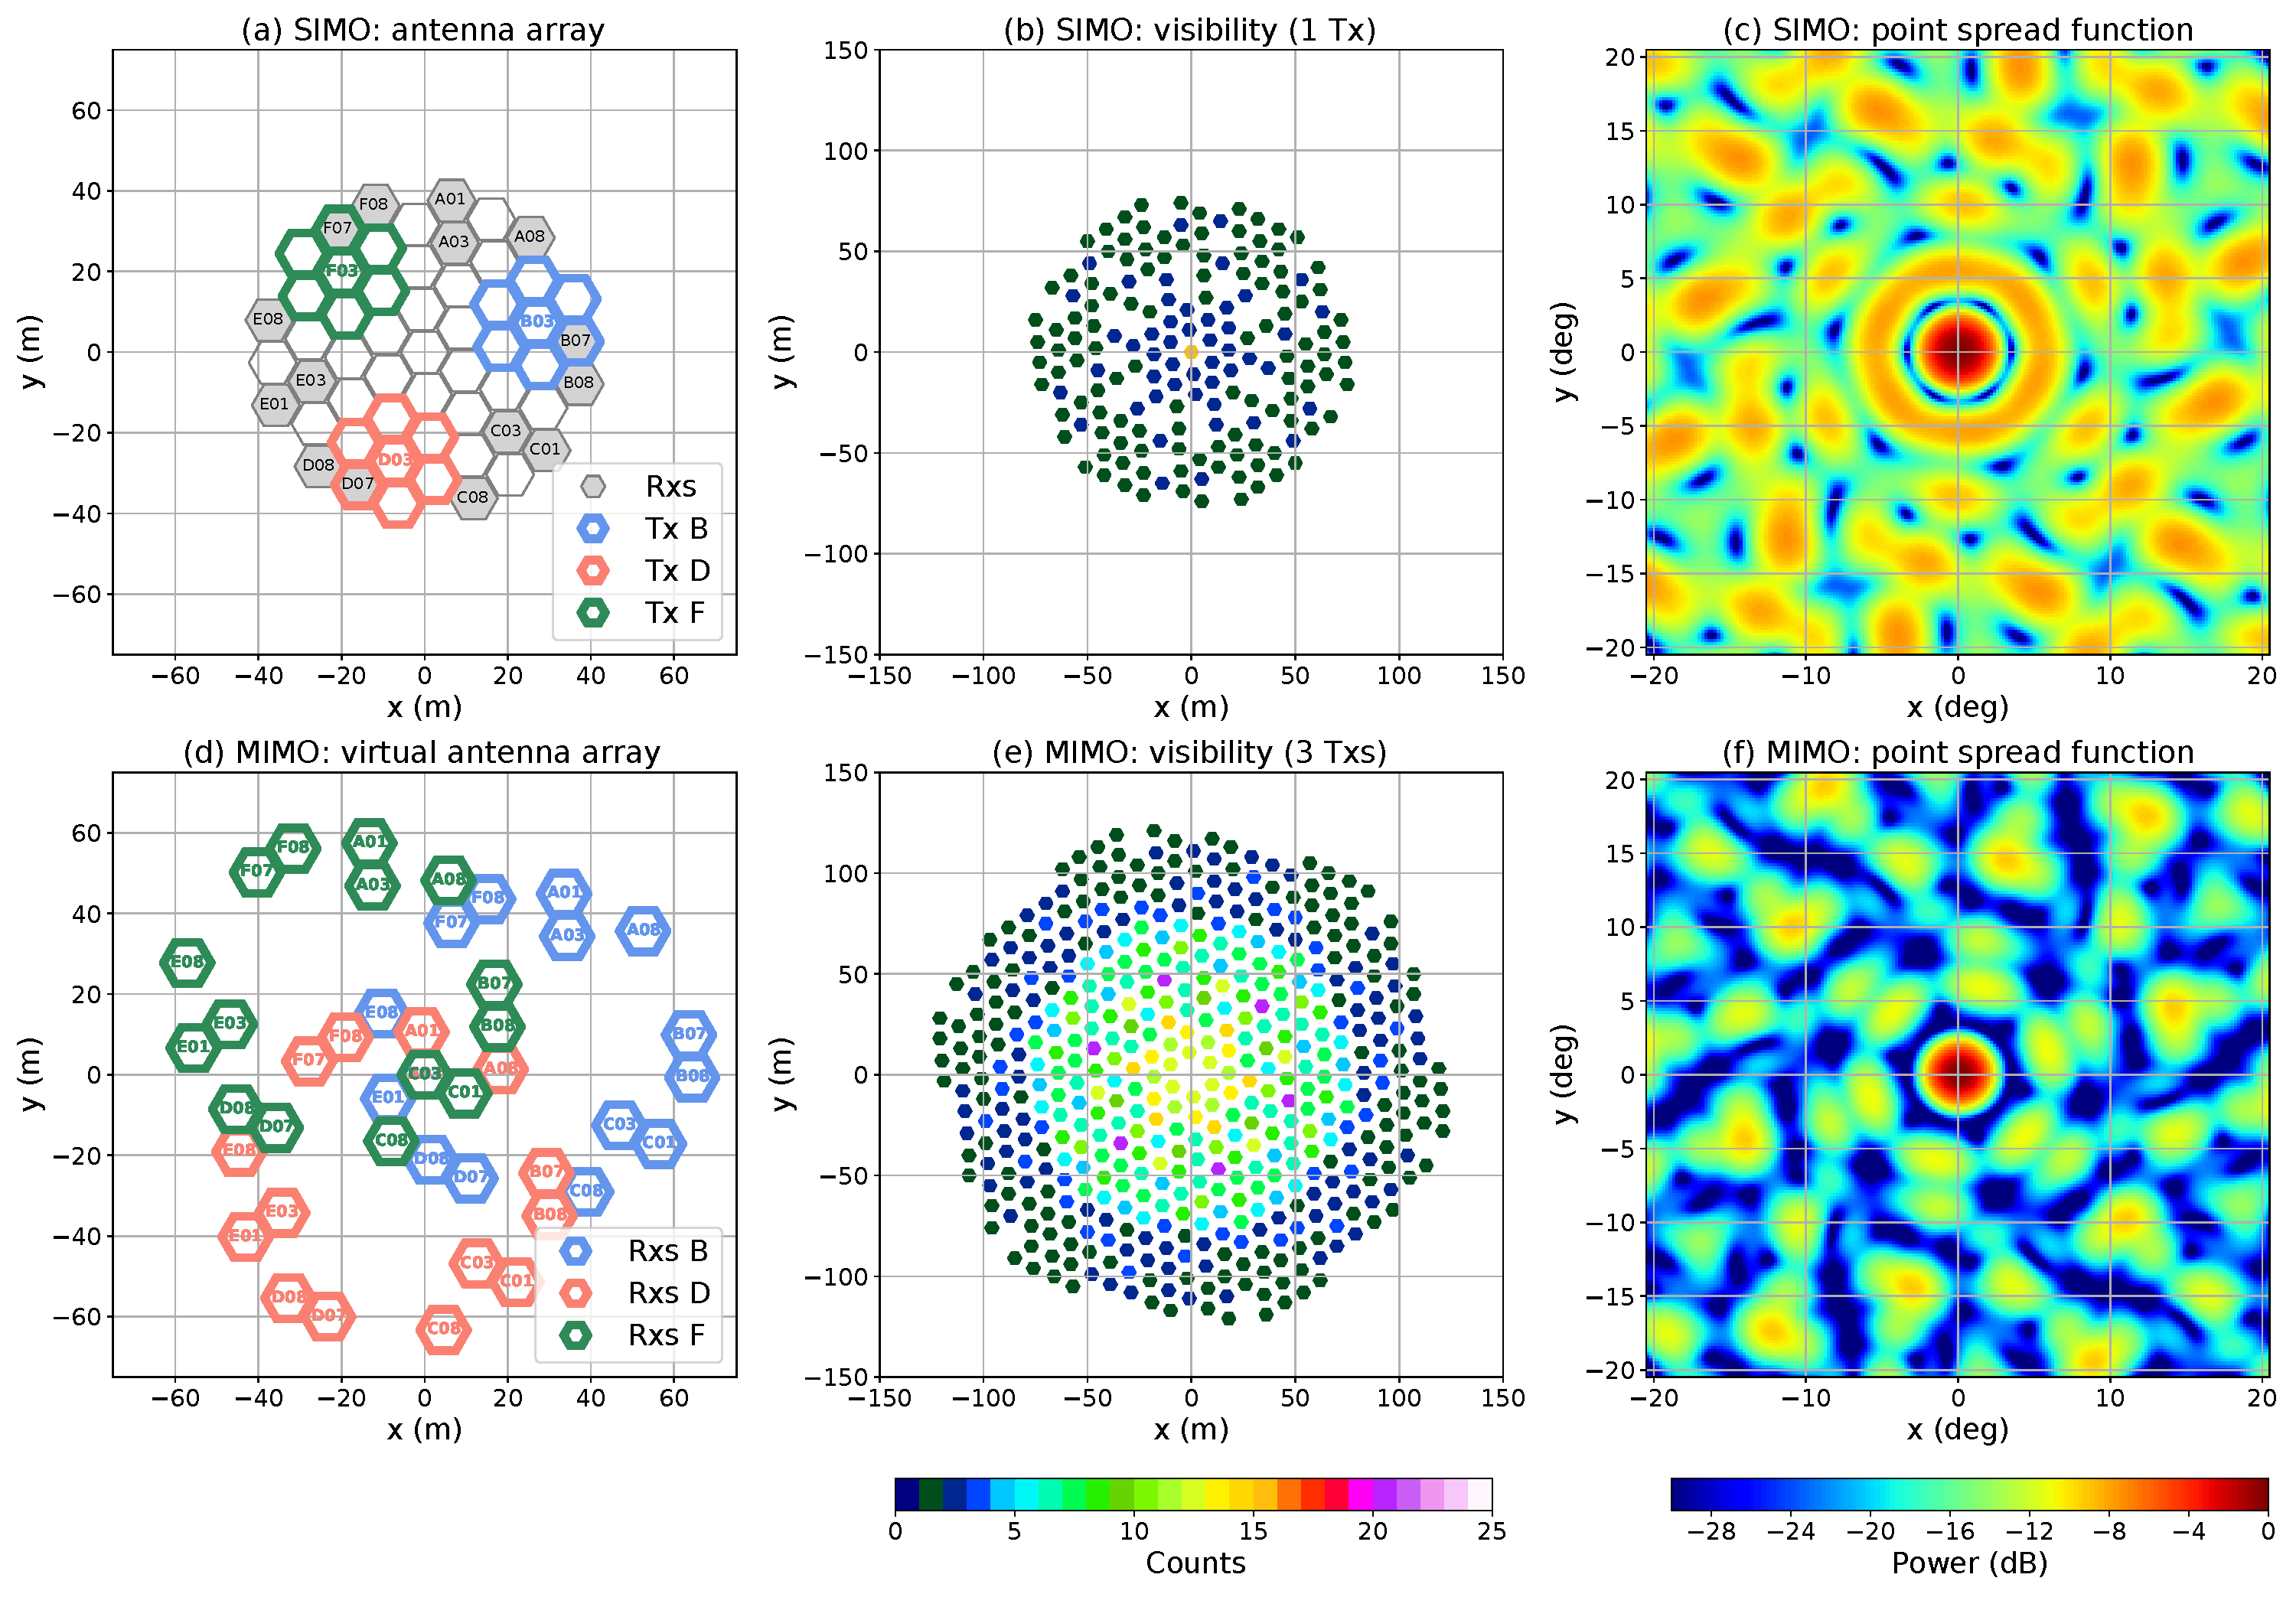
\includegraphics[width=1\linewidth]{figures/amt-12-955-2019-f01-high-res.pdf}
\end{figure}




\vfill

%% Print some more information at the bottom
\begin{tabular}{ll}
    Instructor: & Prof. Gamal Abd El-Fadeil\\
    &Prof. Ahmed Abd El-Halem\\
    Teaching Assistant: & Eng. Basma Diaa \\
    Project Duration: & February , 2026 - Month, 2026 \\
    Faculty: & Faculty of Engineering, Capital University
\end{tabular}

\bigskip
\bigskip


\end{center}

% تأكد من إضافة \usepackage[export]{adjustbox} في مقدمة الملف لدعم valign
\begin{tikzpicture}[remember picture, overlay]
	\node[above=10mm] at (current page.south) {%
		
\includegraphics[width=2.5cm, valign=m]{figures/englogo}  
		
\includegraphics[width=3.5cm, valign=m]{figures/unilogo}
	};
\end{tikzpicture}

\end{titlepage}

%\chapter*{Preface}
\addcontentsline{toc}{chapter}{Preface}

\begin{flushright}
{\makeatletter\itshape
    \@author \\
    Capital, \monthname{} \the\year{}
\makeatother}
\end{flushright}

My choice of engineering stemmed from a childish perspective I had as a child. I imagined engineering students are like scientists in science fiction movies.

But the reality of the two and a half years I spent in engineering college proved me that engineering (at least in Egypt) isn't much different from any other field.

I discovered that (just like in school) I'm studying to pass exams. It doesn't matter how well you understood the material; what matters is your ability to solve specific problems in a particular way. No creativity. No innovation. Nothing interesting.

This project might revive that childish perspective; it might prove that I wasn't 100\% wrong.

The past two years might have been preparation for what's to come, which might align with my old perception. who knows?

For the past two years, I've tried to force the education system to meet my expectations. But the system is bigger than me and everyone else. If it were that simple, everyone would do it.

Therefore, this is my last chance to try and live the experience I've looked for. If it doesn't work, I'll look for a field alongside engineering to fulfill my desire, and to be my way to earn money.

I hope my message, which I consider more important than the research, gets through.

I wrote this preface before starting the research, and I hope to achieve a result beyond my expectations.
\chapter*{Summary}

This project aims to delve into the concept of antenna arrays, focusing specifically on Single Input Multi-Output (SIMO) systems and the differences between them and other systems.

The project is a MATLAB implementation of several communication systems by building the Tx, Rx, and channel in a computational simulation environment.

First, we will discuss the properties of the wave and the reasons that cause radio waves to change shape into beams in Spatial Diversity systems. Then, we will create a semi-realistic environment in communication systems on computer simulation.

Next, using the same environment we created, we will simulate the SISO, SIMO, MISO, and MIMO systems in the case of Line Of Sight channel (LOC) to understand the fundamental differences between them.

after that we will build a multi-path channel to study the effect of it on a SIMO and MIMO systems to see the difference between them.

\tableofcontents
%\listoffigures
%\listoftables

\chapter*{Nomenclature}
\addcontentsline{toc}{chapter}{Nomenclature}

\section*{Abbreviations}



\begin{longtable}{p{2.5cm}p{8cm}}
    \toprule
    Abbreviation & Definition \\
    \midrule\endhead
    \Tx          & Transmitter\\
    \Rx          & Receiver\\
    LOC          & Line Of Sight\\
    SISO         & Single Input Single Output\\
    SIMO         & Single Input Multiable Output\\
    MIMO         & Multiable Input Multiable Output\\
    SNR          & Signal to Noise Ratio \\
    BER          & Bit Error Rate\\
    \bottomrule
\end{longtable}

\section*{Symbols}

\begin{longtable}{p{2.5cm}p{8cm}p{2.5cm}}
    \toprule
    Symbol & Definition & Unit \\
    \midrule\endhead
    $c$ & speed of light & $m/s$ \\
    \midrule
    $\lambda$ & Wavelength & $m$ \\
    \midrule
    $f$ & frequency & $Hz$\\
    \midrule
    B & bandwidth   & $Hz$\\
    \bottomrule
\end{longtable}


%% ----------------------------------------------------------------------
%%    Mainmatter (Arabic page numbering)
%% ----------------------------------------------------------------------

\mainmatter

\chapter{Wave Propagation}
\label{chapter:introduction}

Before talking about antennas,
we must first understand some things about how a wave propagates in space.

\section{Huygens principle}
\begin{wrapfigure}{r}{0.35\textwidth}
	\centering
	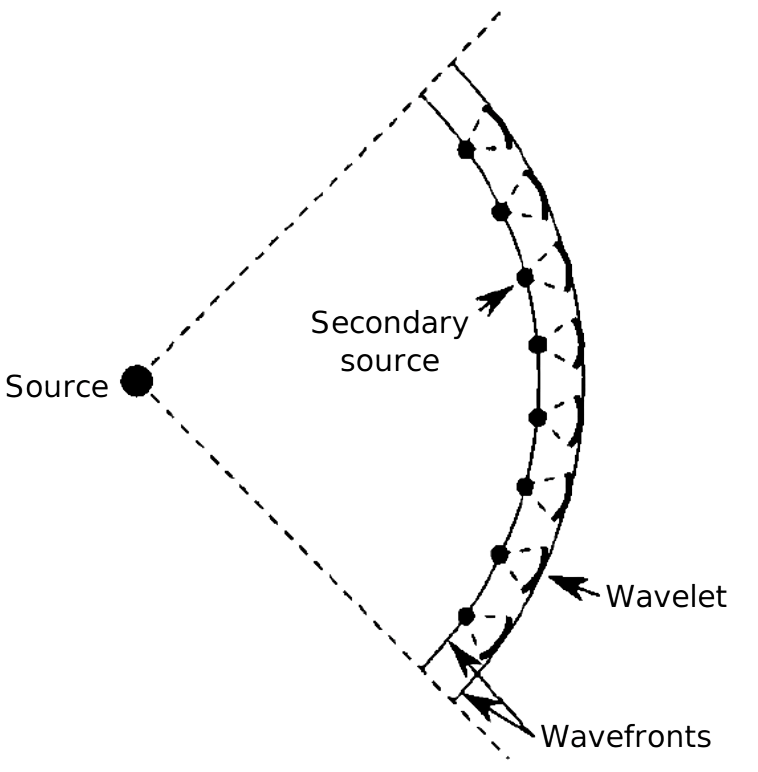
\includegraphics[width=0.35\textwidth]{figures/1.png}
	\caption{}
	\label{1}
	\vspace{1cm}
	
\includegraphics[width=0.35\textwidth]{figures/wave-diffraction}
	\caption{}
	\label{2}
\end{wrapfigure}

Huygens' principle states that every point on a wave can be considered as a source of a wave.

As clearly shown in [Figure \ref{1}], after the wave spreads from the main source, each point on the wave acts as a source of waves. However, since the points composing the wave are theoretically infinite, the sum of the waves generated by all these points results in a smooth wave without distortions.

\section{Wave diffraction}
Therefore, when a wave hits a barrier, part of the wave (part of the wave sources) passes through, and a phenomenon called wave diffraction [Figure \ref{2}] occurs.

When the wave passes through a very small slit, a wave is produced on the other side of the barrier in the shape of a semicircle (or a hemisphere if we look at it from a three-dimensional perspective).

\section{Double slit experiment}
This is one of the most famous experiments in modern physics and quantum mechanics. However, we will discuss the experiment from a wave perspective only.

When a wave passes through two slits, each slit allows a small portion of the wave to pass through. This portion behaves as a single-point wave source, creating a semicircular wave.

The two waves intersect, creating areas where in phase regions intersect, increasing the wave's amplitude (constructive interference). 
Conversely, out-of-phase regions intersect, decreasing the wave's amplitude (destructive fading), as we can see Figure[\ref{fig:double-slit}], the amplitude of the beam in the middle is the most saturated one, and we loss saturation gradually surrounding beams as we go further away.

\newpage
\begin{figure}[!h]
	\centering
	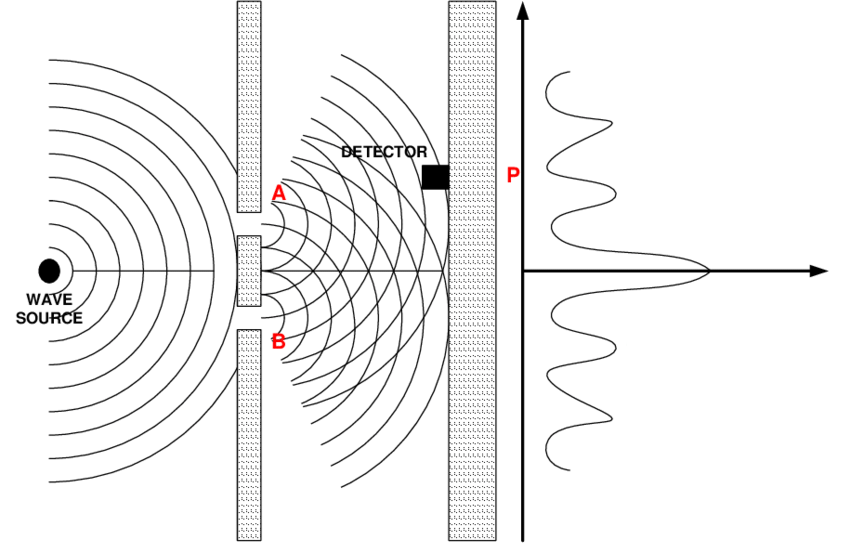
\includegraphics[width=0.7\linewidth]{figures/Double-slit-experiment-illustrating-the-wave-behavior-of-light}
	\caption{}
	\label{fig:double-slit}
\end{figure}

\section{antenna array}
In the previous experiment, we used only two wave sources in a three-dimensional space.

In a commercial antenna array, we use more than two wave sources (antennas) arranged on a three-dimensional surface. In this case, we get a set of beams, as happened in the double-slit experiment. However, as the number of antennas in the array increases, the concentration of the beam in the center (main lobe) increases at the expense of the side beams (side lodes).

This makes the wave emitted by the antenna somewhat similar to a laser. Figure[\ref{fig:1532895074001}].

the beam in the middle has much more SNR than a single antenna with the same power of the system will have in the same distance.
so we use this phenomenon to decrease the probability of error of the system so we can decrease the BER.

\begin{figure}[!h]
	\centering
	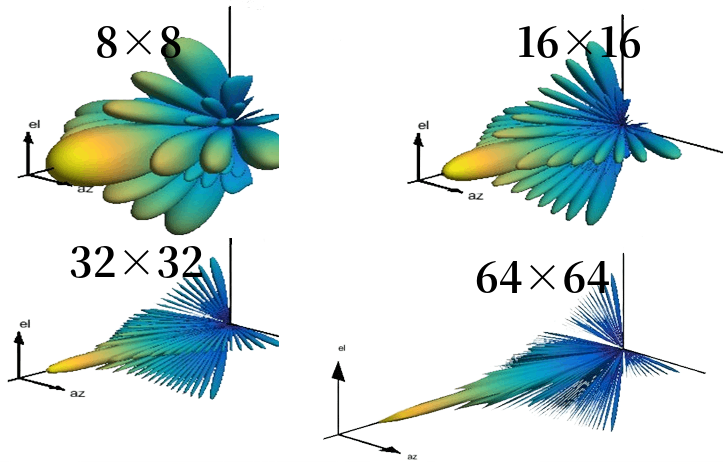
\includegraphics[width=0.6\linewidth]{figures/beams}
	\caption{}
	\label{fig:1532895074001}
\end{figure}

\newpage
\section{Spatial Diversity}
it's the process of staking more then one array it the \Tx (MISO) or the \Rx (SIMO) or both of them (MIMO) to decrease the probability of error of the communication system and to concentrate the wave into a beam in a directed angle.


Figure[\ref{fig:spatial-diversity}].
\begin{figure}[!h]
	\centering
	\includegraphics[width=1\linewidth]{"figures/Spatial Diversity"}
	\caption{Spatial Diversity}
	\label{fig:spatial-diversity}
\end{figure}
\chapter{Line Of Sight System Initialization}

before we start anything we need first to initialize and set the the parameters of the environment of our communication system
\section{wave parameters}
we first set the speed of light to be $5\times10^{8} m/s$ and the carrier frequency $f_c$ to be $6\times10^{10} H_z (60 GH_z)$

we can calculate the wave length of the carrier $\lambda_c$ from the relation
$$
\lambda_c = \frac{c}{f_c} = \frac{5\times10^{8}}{6\times10^{10}} = 8.\overline{3} \times10^{-3}
$$
\section{\Tx and \Rx spatial relationship}
after that we set the \Tx and the \Rx in a 3D coordinate to determine the spatial relationship between Them.
\begin{center}
	\Tx center = (~~~0~~~,~~0~~,0)\\
	\Rx center = (1500,500,0)\\
\end{center}

The distance between the centers of \Tx and \Rx is equal to 1581.14 meter.

and because the wave does form into beams in a specific angels we need to specify the angle for both \Tx and \Rx see each other.

we can do so using a function called 'rangeangle' which return the range and the angle between two position vectors, we don't need the range so we will take the second index value only which returns the angle.

\section{Data Generation}
we will use a 1 million random binary sequence as a data to be transmitted in our system from the \Tx to the \Rx.

and we will assign the array to a variable called x (x will represent the original data)

\newgeometry{margin=0pt}
\newpage
\vfill
\begin{figure}
	\centering
	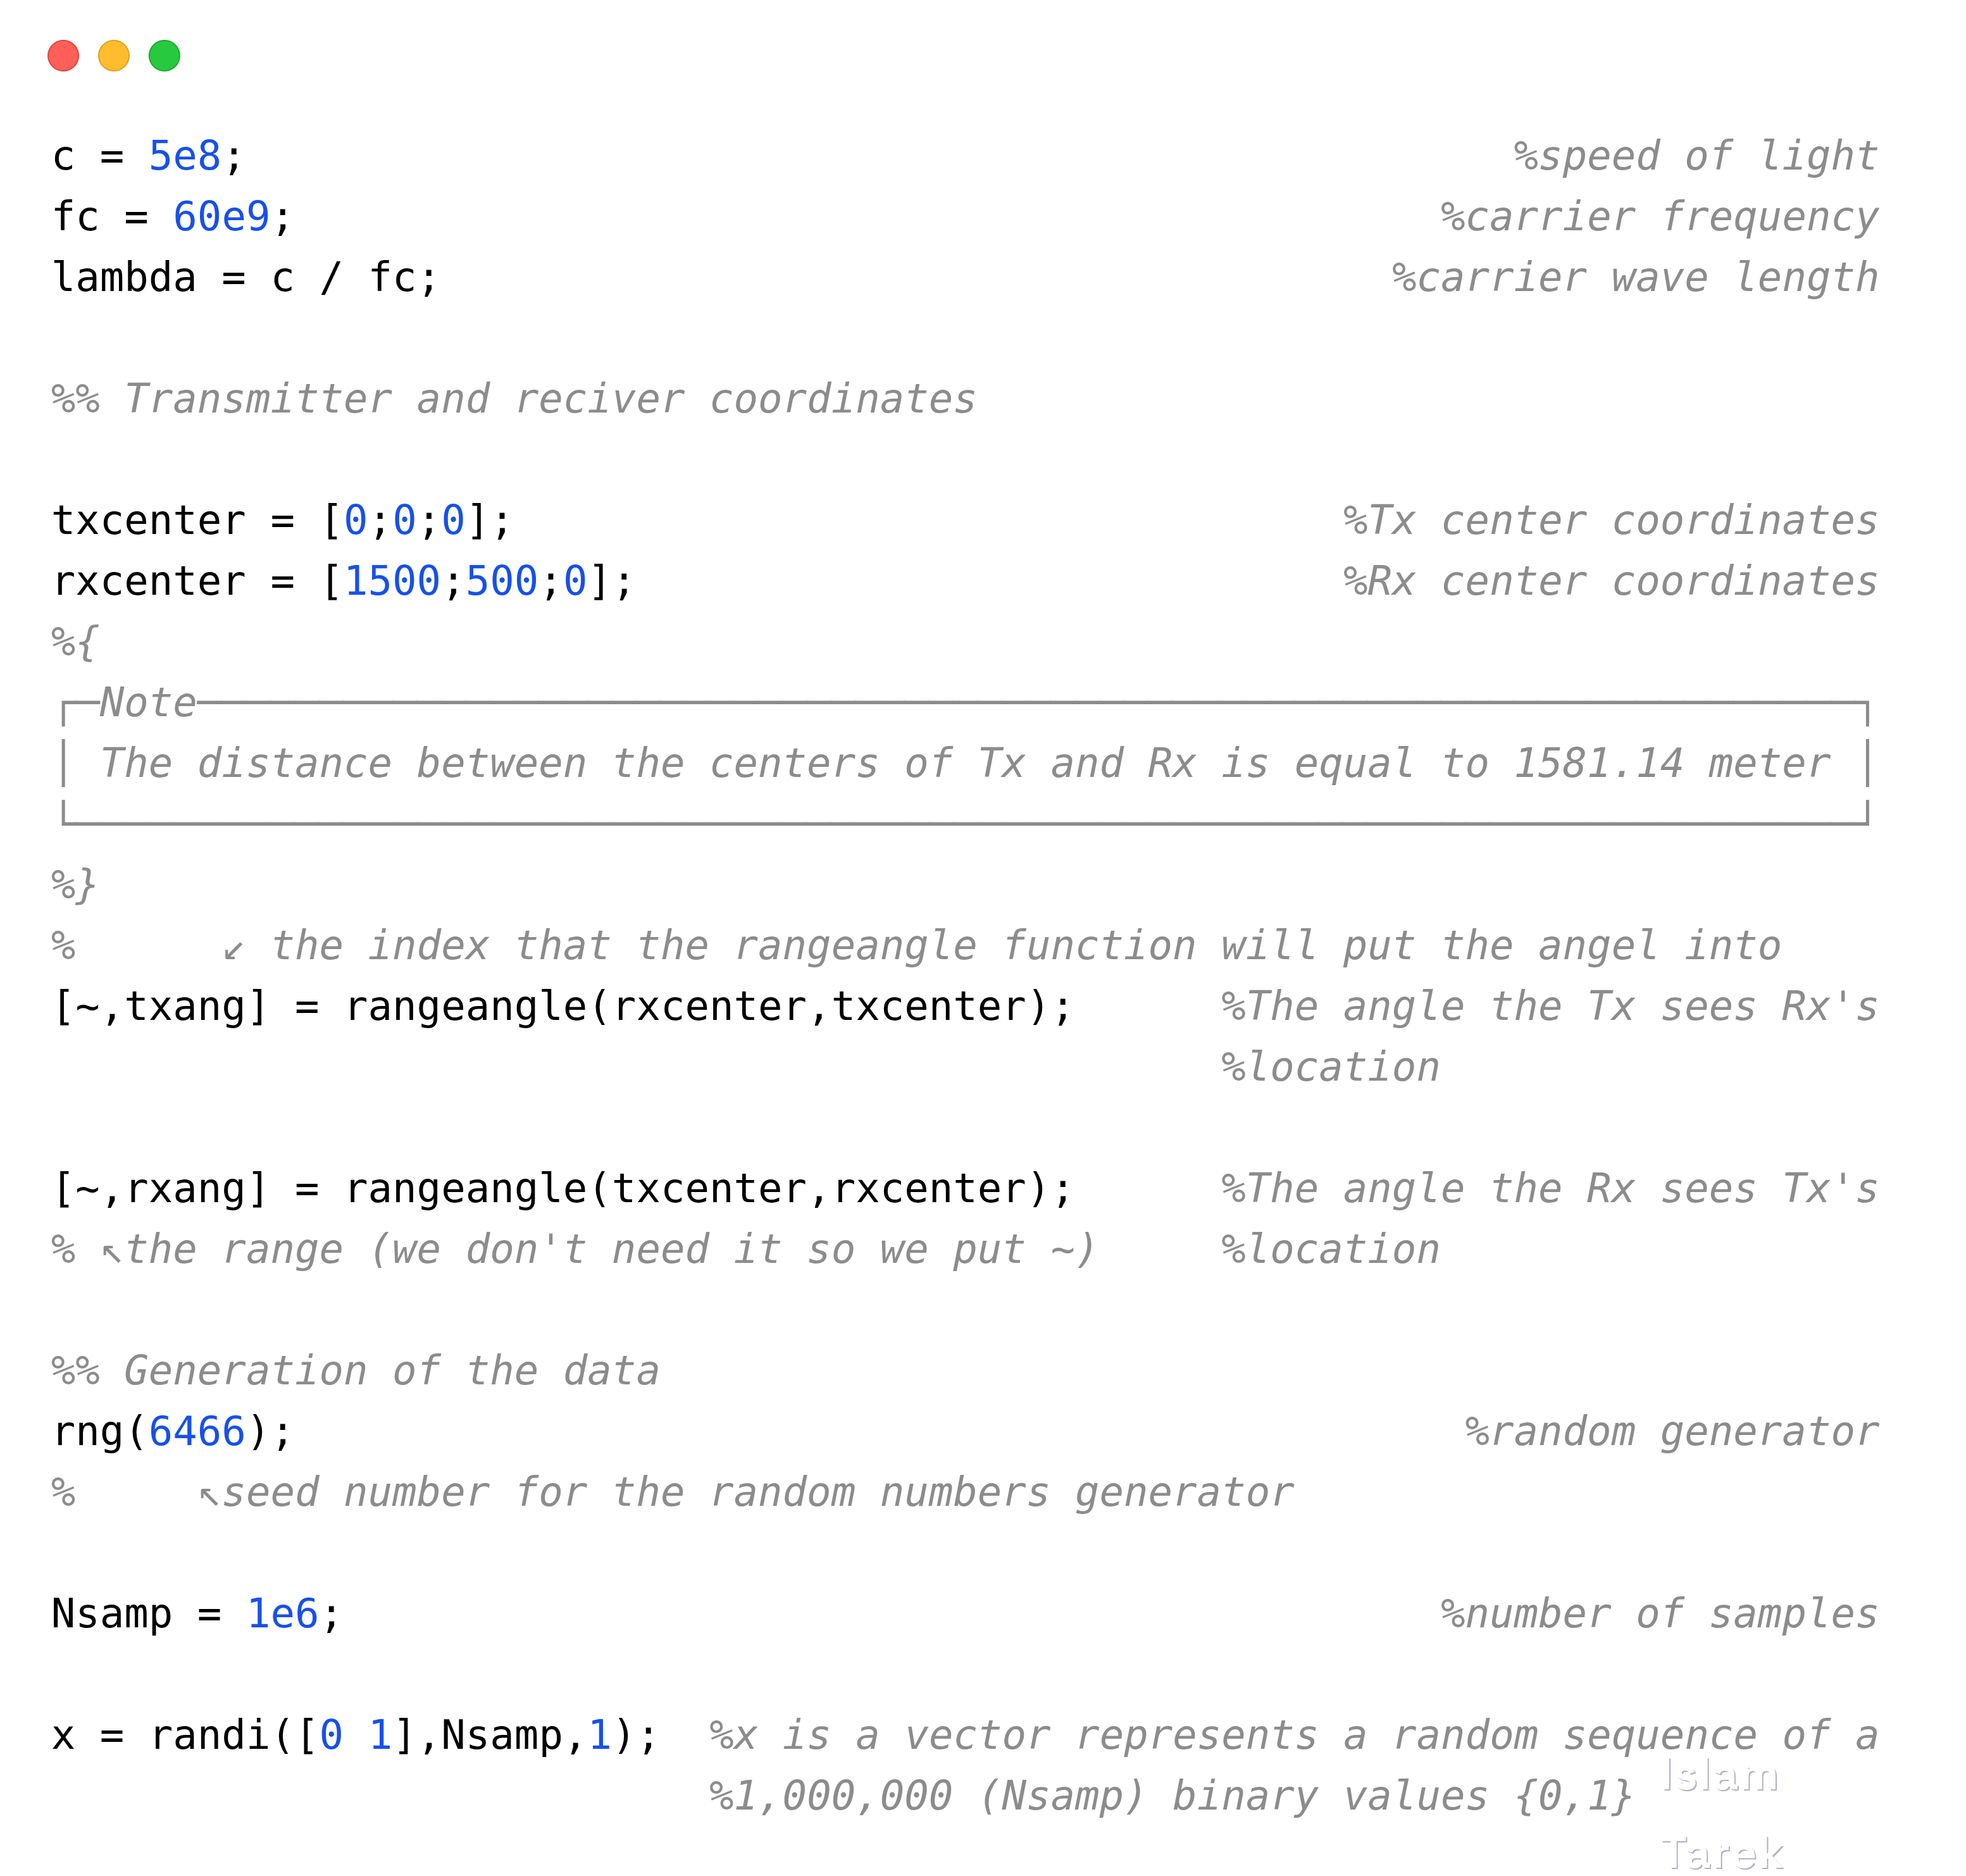
\includegraphics[width=0.8\linewidth]{figures/code1}
\end{figure}
\vfill
\restoregeometry
\chapter{Single Input Single Output Line Of Sight Channel}

this is the simplest way to transmit a signal wirelessly, by using one antenna at both \Tx and \Rx. but this simplicity comes with it's costs.

\section{Antennas position}
for this system we use single antenna at the center of the \Tx and \Rx , which is (0,0,0) for the both proportional to their centers.\\
\Tx single input position $\to$ txsipos = (0,0,0)\\
\Rx single input position $\to$ rxsipos = (0,0,0)\\

\section{Scattering channel matrix}
\subsection{Scattering model}
is a model designed to describe the scattering of a radio waves in complex environments
\subsection{Scatteringchanmtx}
it's a function that generates a matrix that describes the wireless channel by based on the scattering model, by knowing:
\begin{enumerate}
	\item \Tx antenna array
	\item \Rx antenna array
	\item \Tx angle
	\item \Rx angle
	\item channel gain (gain = 1)
\end{enumerate}
\section{Eb/No}
it's the power of a single bit (Eb) divided by the spectral noise power density (No)\\
and it equals
$$
\frac{\text{Eb}}{\text{No}} = \text{SNR} \times \frac{\text{B}}{\text{R}_\text{b}}
$$
in our case we will use 11 different values for it to see the the effects on the communication system for different Eb/No values.

\section{Bit Error Rate (BER)}
it is the number of bit errors divided by the total number of transmitted bits over a given time interval.

in this project, we will calculate it by an assigned function called 'helpMIMOBER' which takes the scattering channel matrix, the original bit sequence (x) and Eb/No to calculate the BER.

in our case we want to monitor the relationship between Eb/No and BER in a SISO LOS channel so will use the 11 values of Eb/No and calculate the BER for each one using helpMIMOBER function.
\section{Plotting}
as we can see in Figure[\ref{fig:sisober}], the BER decreases as we increase the Eb/No.

and it's pretty striate forward, as long as we increase the ratio of the bit power over the noise spectral power, the probability of bit error decreases.

\begin{figure}[!h]
	\centering
	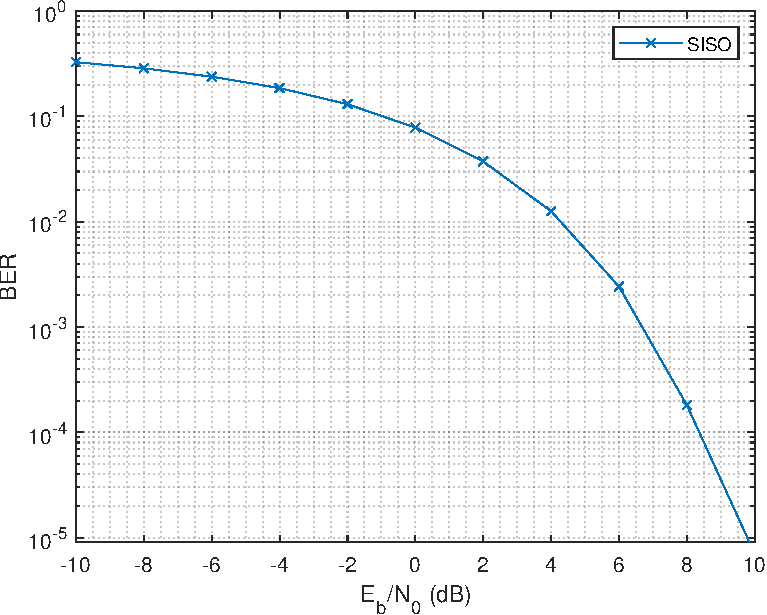
\includegraphics[width=1\linewidth]{figures/SISO_BER}
	\caption{SISO BER for each Eb/No}
	\label{fig:sisober}
\end{figure}



\newgeometry{margin=0pt}
\newpage
\vfill
\begin{figure}
	\centering
	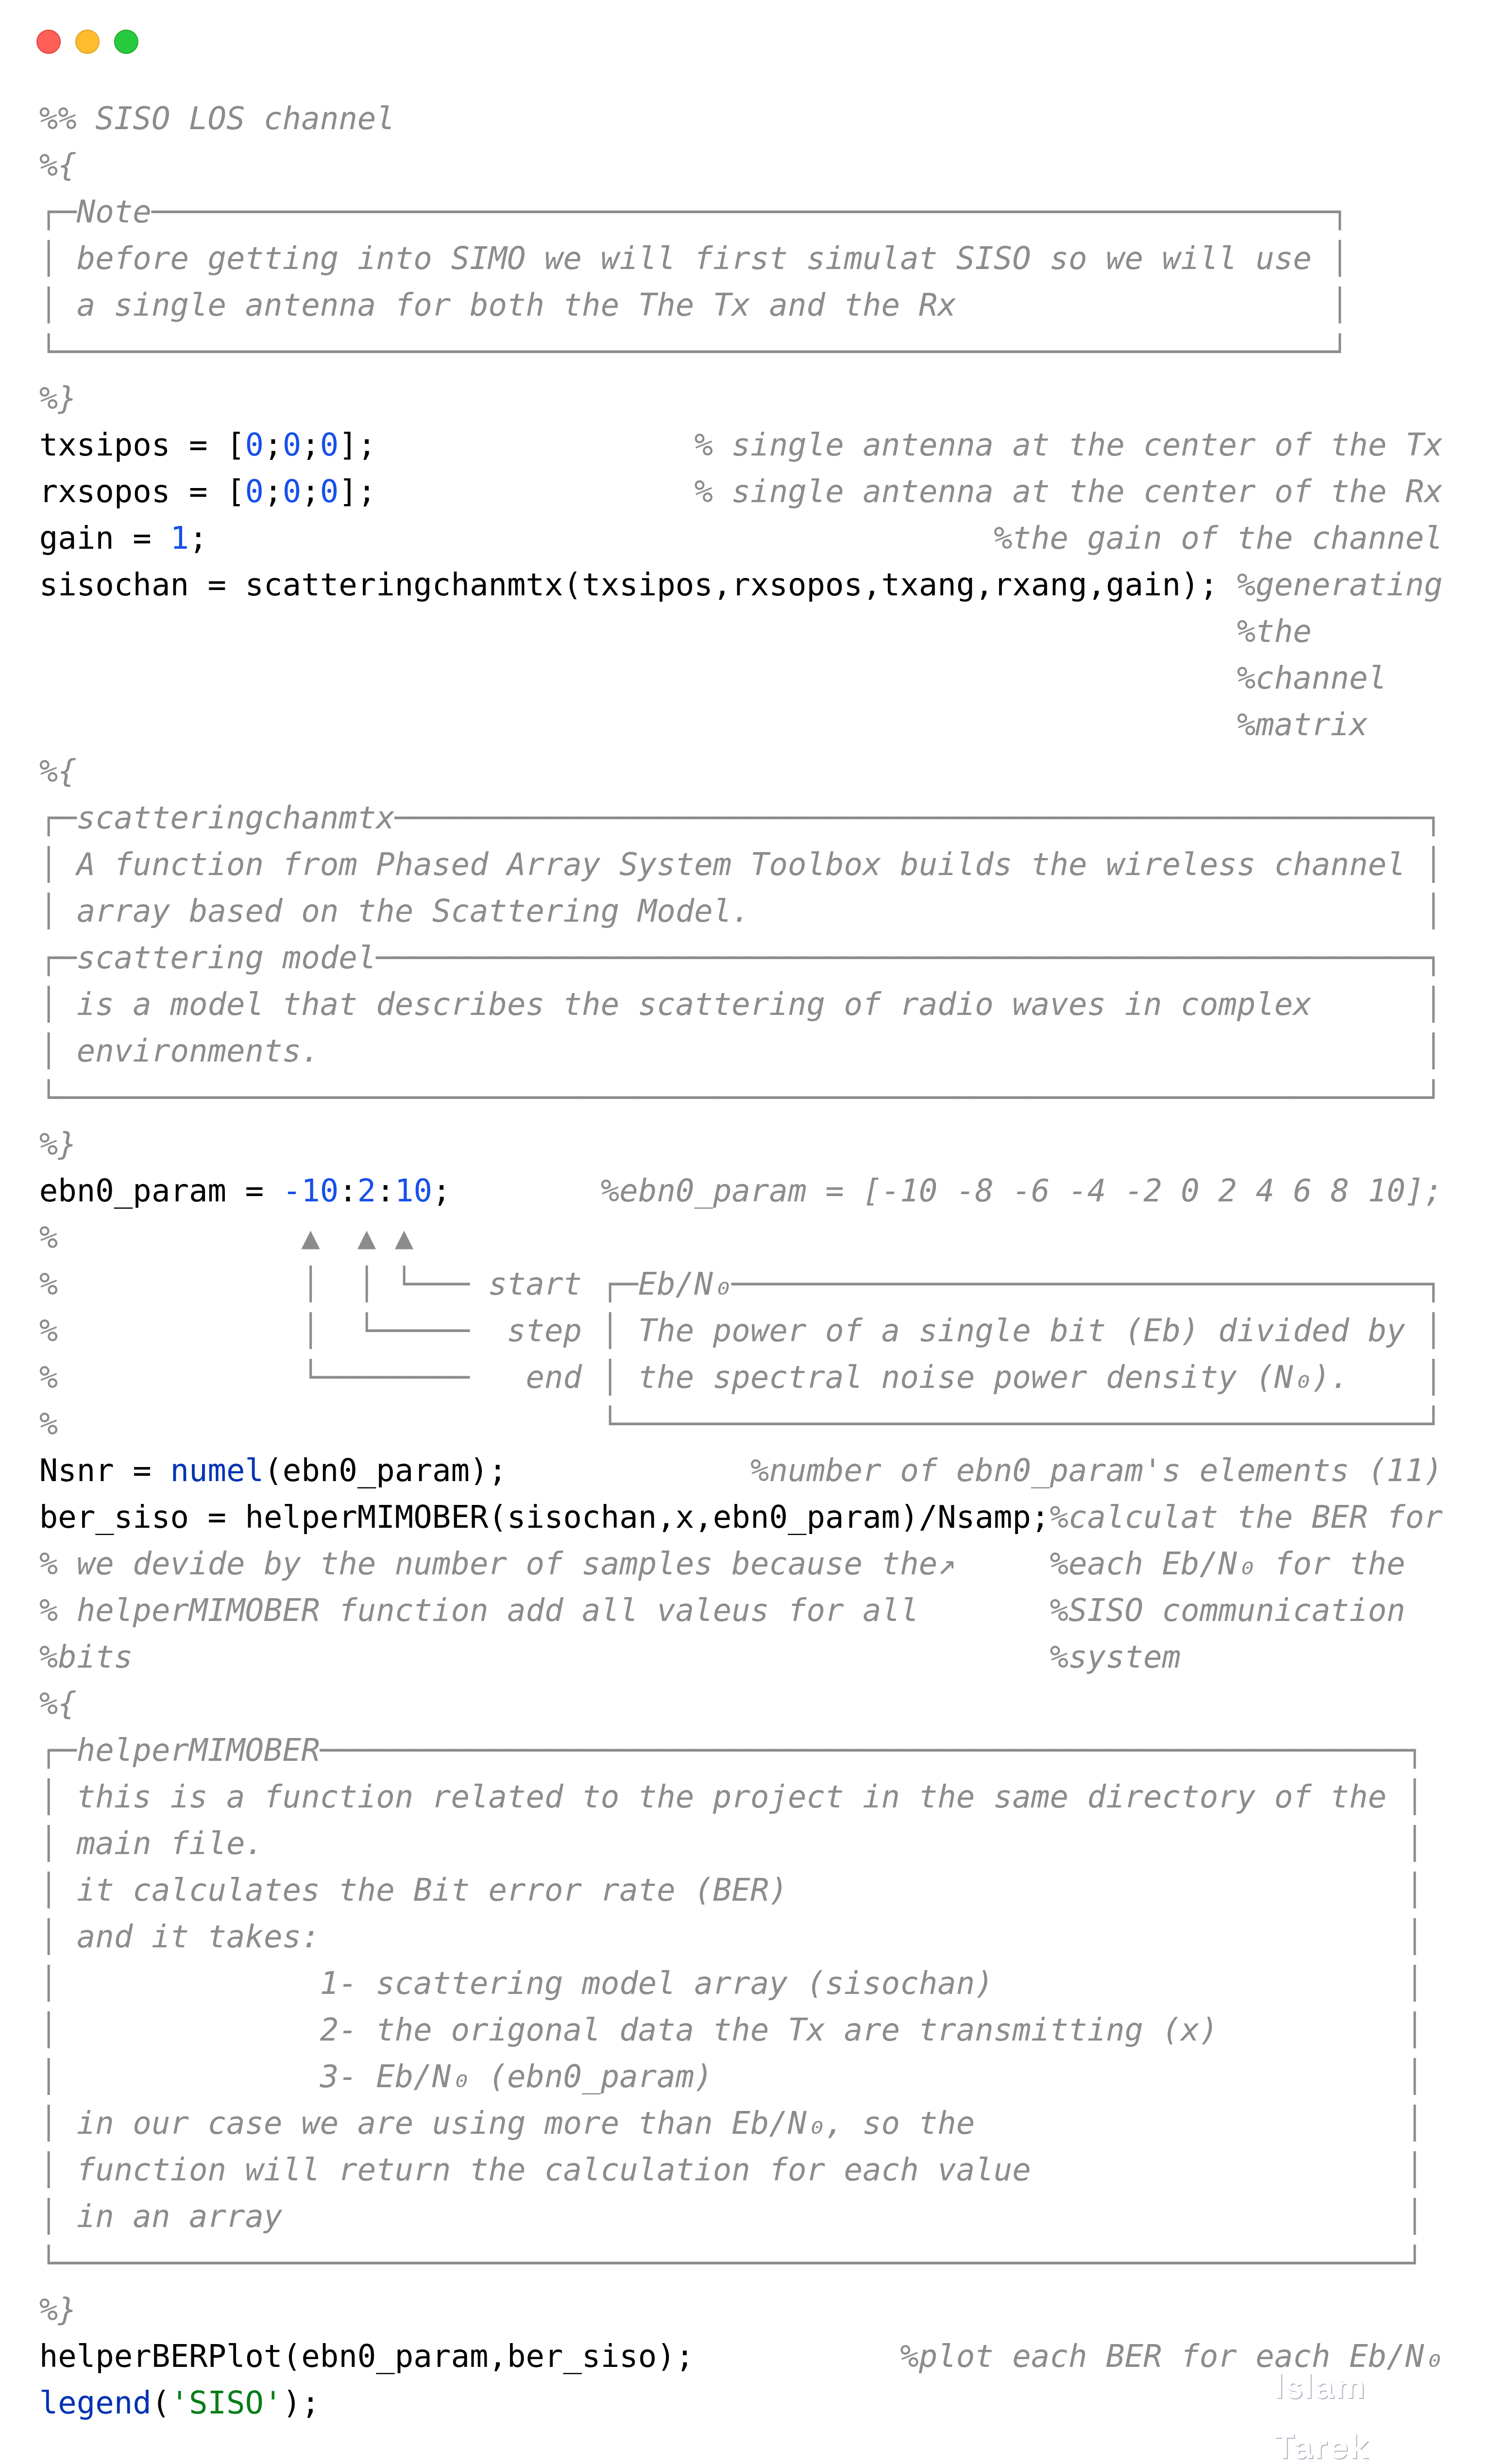
\includegraphics[width=0.8\linewidth]{figures/code2}
\end{figure}
\vfill
\restoregeometry
\chapter{Single Input Multiple Output Line of Sight Channel}

this system uses a multiple antennas at the \Rx to decrease the probability of error in the communication system, and that's a type of Spatial Diversity.

\section{\Rx antenna array}
in a SIMO communication system, we send the message from a \Tx with one antenna and receive it with multiable antennas \Rx.

the structure (the way the antennas are arranged) called the antenna array.
by using the two built-in functions 'phased.ULA' and 'getElementPosition', we can make a liner antenna array and get the coordinates for each antenna.

\subsection{Scatteringchanmtx}
as we did in SISO LOS, we will repeat it for each system because we need scattering channel matrix to calculate the BER.
the difference here is we will replace the single antenna we put as the \Rx with the antenna array we made in the previous step.

\section{Bit Error Rate (BER)}
we will calculate it this time for the SIMO system.

to monitor the relationship between Eb/No and BER in a SIMO LOS channel so will use the 11 values of Eb/No and calculate the BER for each one using helpMIMOBER function.
\vfill

\begin{figure}[!h]
	\centering
	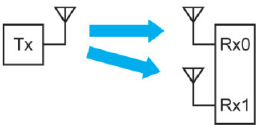
\includegraphics[width=0.4\linewidth]{figures/SIMO}
	\caption{SIMO}
\end{figure}

\newpage
\section{Plotting}
to see the difference between SISO and SIMO we will plot the both of them on the same graph.

as we can see in Figure[\ref{SISO and SIMO BER for each Eb/No}], the BER decreases as we increase the Eb/No for each SISO and SIMO.

but the SIMO curve is steeper than the SISO one, which indicates a better BER for SIMO over SISO.

\begin{figure}[!h]
	\centering
	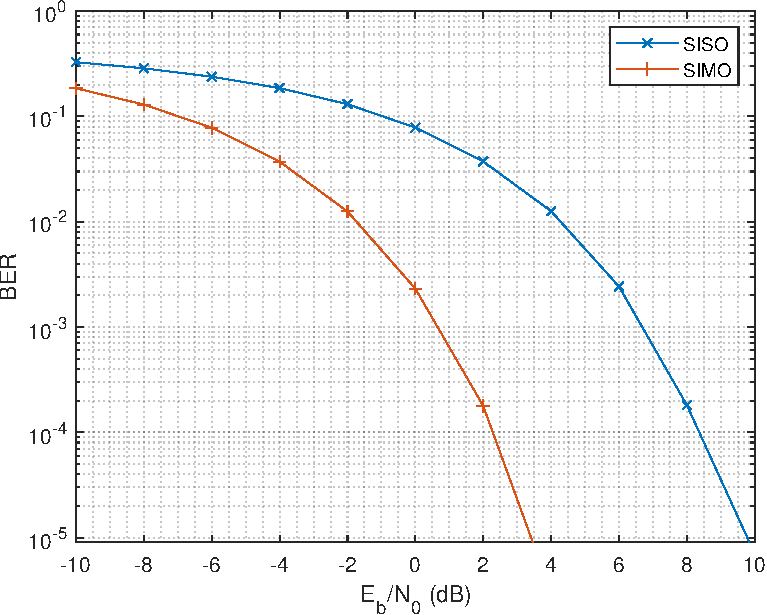
\includegraphics[width=1\linewidth]{figures/SISO_SIMO_BER}
	\caption{}
	\label{SISO and SIMO BER for each Eb/No}
\end{figure}


\newgeometry{margin=0pt}
\newpage
\vfill
\begin{figure}
	\centering
	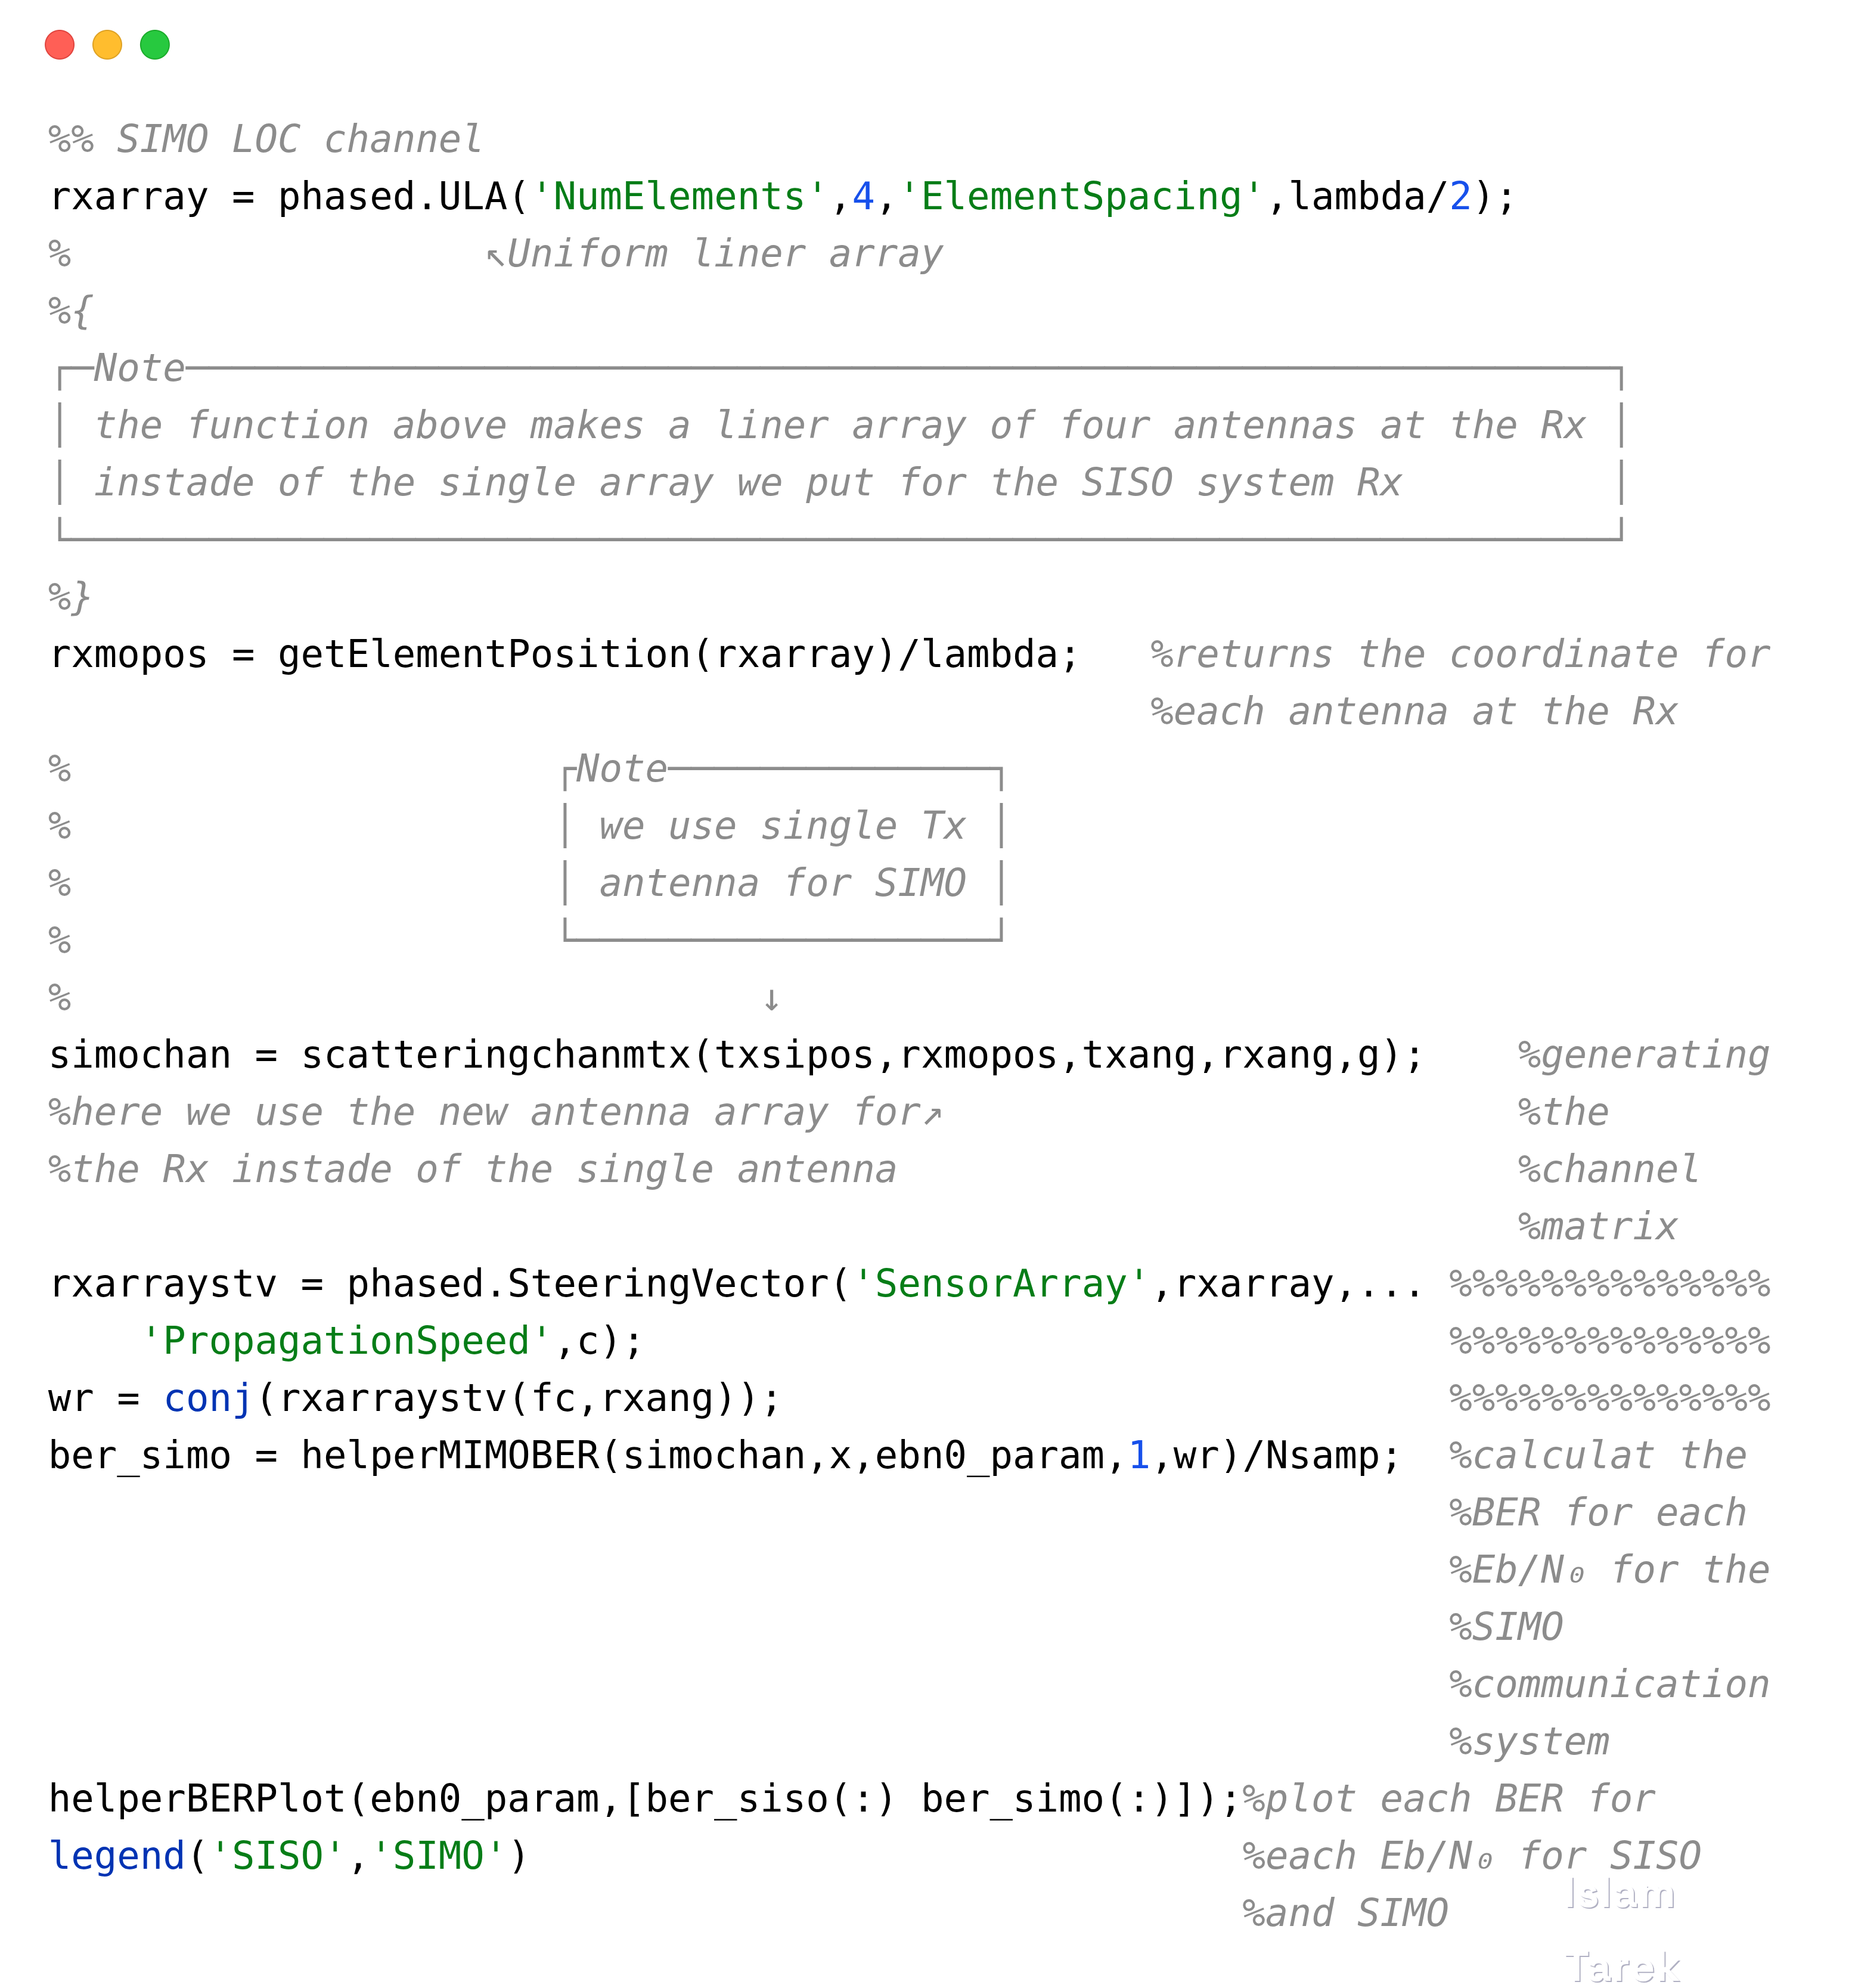
\includegraphics[width=0.7\linewidth]{figures/code3}
\end{figure}
\vfill
\restoregeometry
\chapter{Multiple Input Single Output Line Of Sight Channel}

this system uses a multiple antennas at the \Tx to decrease the probability of error in the communication system, and that's a type of Spatial Diversity.

\section{\Rx antenna array}
in a MISO communication system, we send the message from a \Rx with one antenna and receive it with multiable antennas \Tx.

the structure (the way the antennas are arranged) called the antenna array.
by using the two built-in functions 'phased.ULA' and 'getElementPosition', we can make a liner antenna array and get the coordinates for each antenna.


\subsection{Scatteringchanmtx}
as we did in SISO and SIMO LOS, we will repeat it for each system because we need scattering channel matrix to calculate the BER.
the difference here is we will replace the single antenna we put as the \Tx with the antenna array we made in the previous step.
and the \Rx will be one antenna as it was in SISO.

\section{Bit Error Rate (BER)}
we will calculate it this time for the MISO system.

to monitor the relationship between Eb/No and BER in a MISO LOS channel so will use the 11 values of Eb/No and calculate the BER for each one using helpMIMOBER function.

\vfill
\begin{figure}
	\centering
	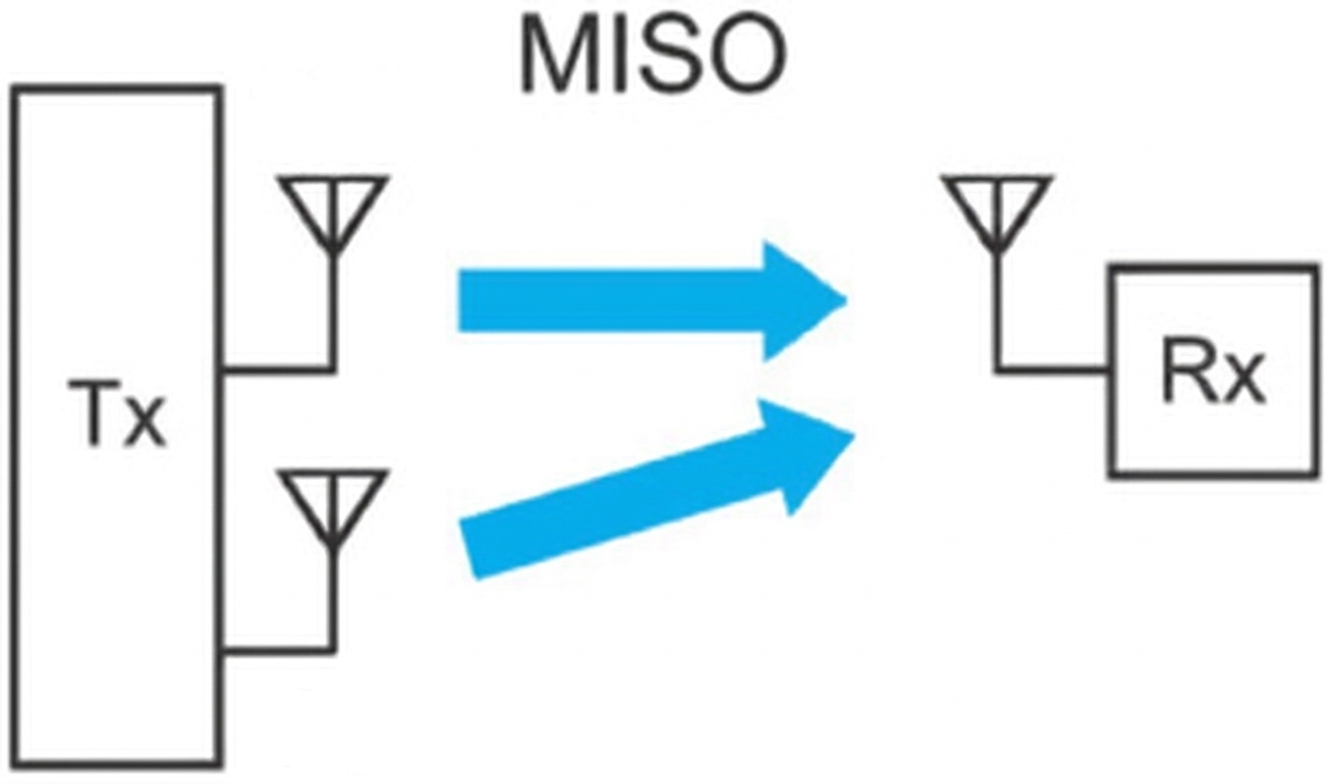
\includegraphics[width=0.4\linewidth]{figures/MISO-gem}
	\caption{MISO}
\end{figure}


\newpage
\section{Plotting}
to see the difference between SISO, SIMO and MISO we will plot all of them on the same graph.

as we can see in Figure[\ref{fig:sisosimomisober}], the BER decreases as we increase the Eb/No for each SISO, SIMO and MISO.

\section{Why do we see only two curves}
the graphs monitored on Figure[\ref{fig:sisosimomisober}] should have been three graph, because we are plotting 3 relations for three systems (SISO, SIMO and MISO).
but because the relation between Eb/No and BER for SIMO and MISO are identical, they overlap each other so we can only see SISO curve and the overlapping SIMO, MISO curev.


\begin{figure}[!h]
	\centering
	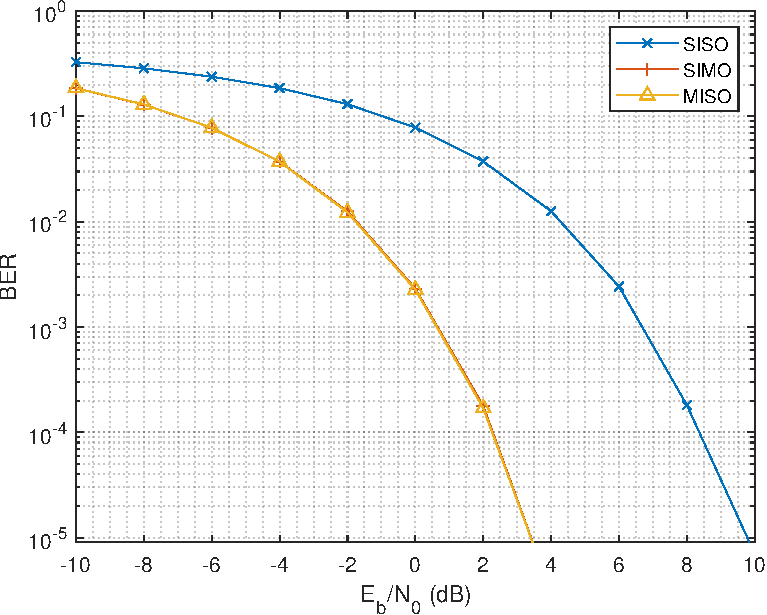
\includegraphics[width=1\linewidth]{figures/SISO_SIMO_MISO_BER}
	\caption{}
	\label{fig:sisosimomisober}
\end{figure}



\newgeometry{margin=0pt}
\newpage
\vfill
\begin{figure}
	\centering
	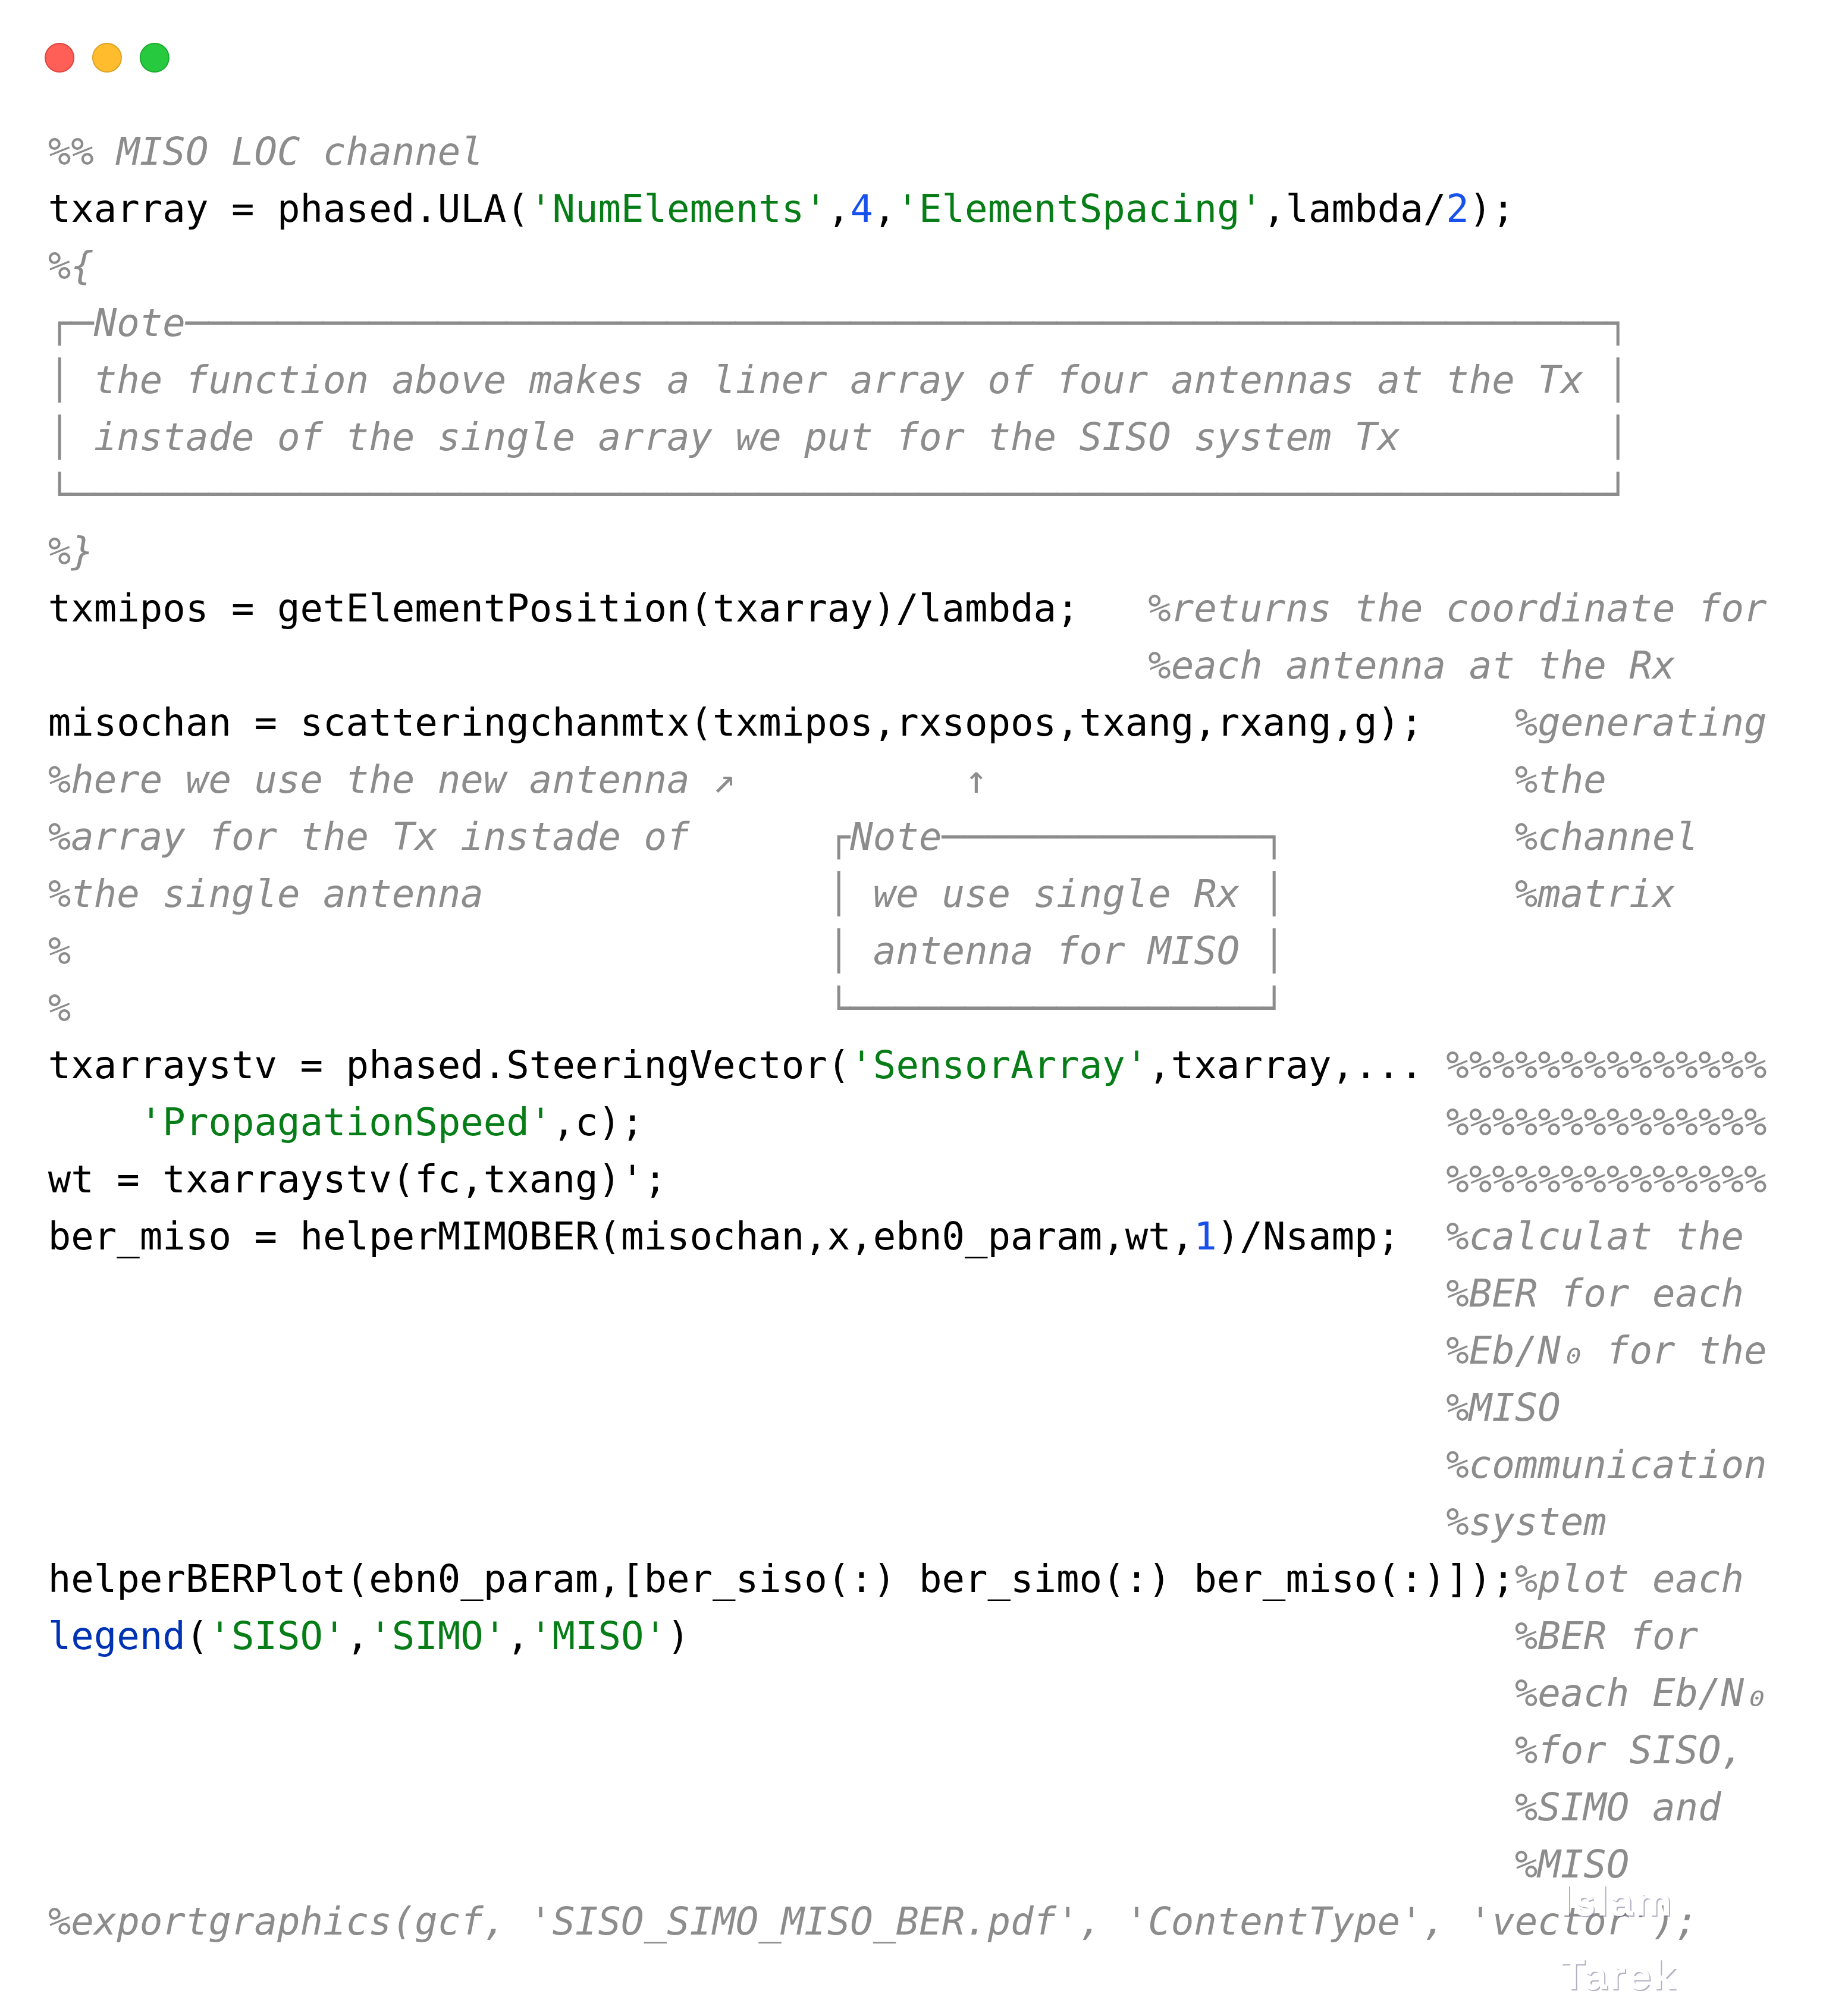
\includegraphics[width=0.7\linewidth]{figures/code4}
\end{figure}
\vfill
\restoregeometry
\chapter{Multiple Input Multiple Output Line Of Sight Channel}

this system uses a multiple antennas at the \Tx and \Rx to decrease the probability of error in the communication system, and that's a type of Spatial Diversity.

\section{\Tx \& \Rx antenna arrays}
we already defined those arrays in MISO and SIMO systems, we we will just call them back again.


\subsection{Scatteringchanmtx}
as we did in SISO, SIMO and MISO LOS, we will repeat it for this system because we need scattering channel matrix to calculate the BER.
the difference here is we will place the antenna array we made at both \Tx and \Rx.

\section{Bit Error Rate (BER)}
we will calculate it this time for the MIMO system.

to monitor the relationship between Eb/No and BER in a MIMO LOS channel so will use the 11 values of Eb/No and calculate the BER for each one using helpMIMOBER function.

\vfill
\begin{figure}
	\centering
	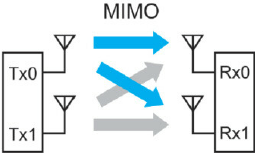
\includegraphics[width=0.4\linewidth]{figures/MIMO}
	\caption{MISO}
\end{figure}


\newpage
\section{Plotting}
to see the difference between SISO, SIMO (or MISO) and MIMO we will plot all of them on the same graph.

as we can see in Figure[\ref{fig:sisosimomimober}], the BER decreases as we increase the Eb/No for each SISO, SIMO and MIMO.


\begin{figure}[!h]
	\centering
	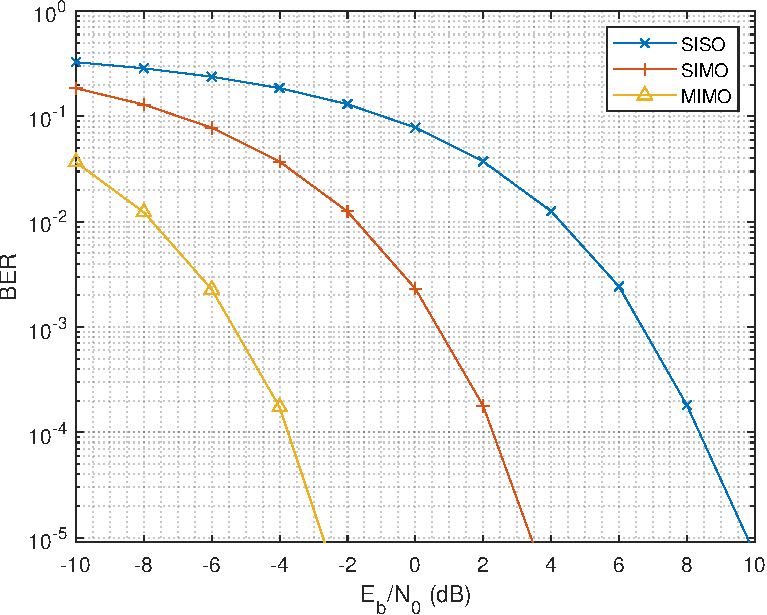
\includegraphics[width=1\linewidth]{figures/SISO_SIMO_MIMO_BER}
	\caption{}
	\label{fig:sisosimomimober}
\end{figure}



\newgeometry{margin=0pt}
\newpage
\vfill
\begin{figure}
	\centering
	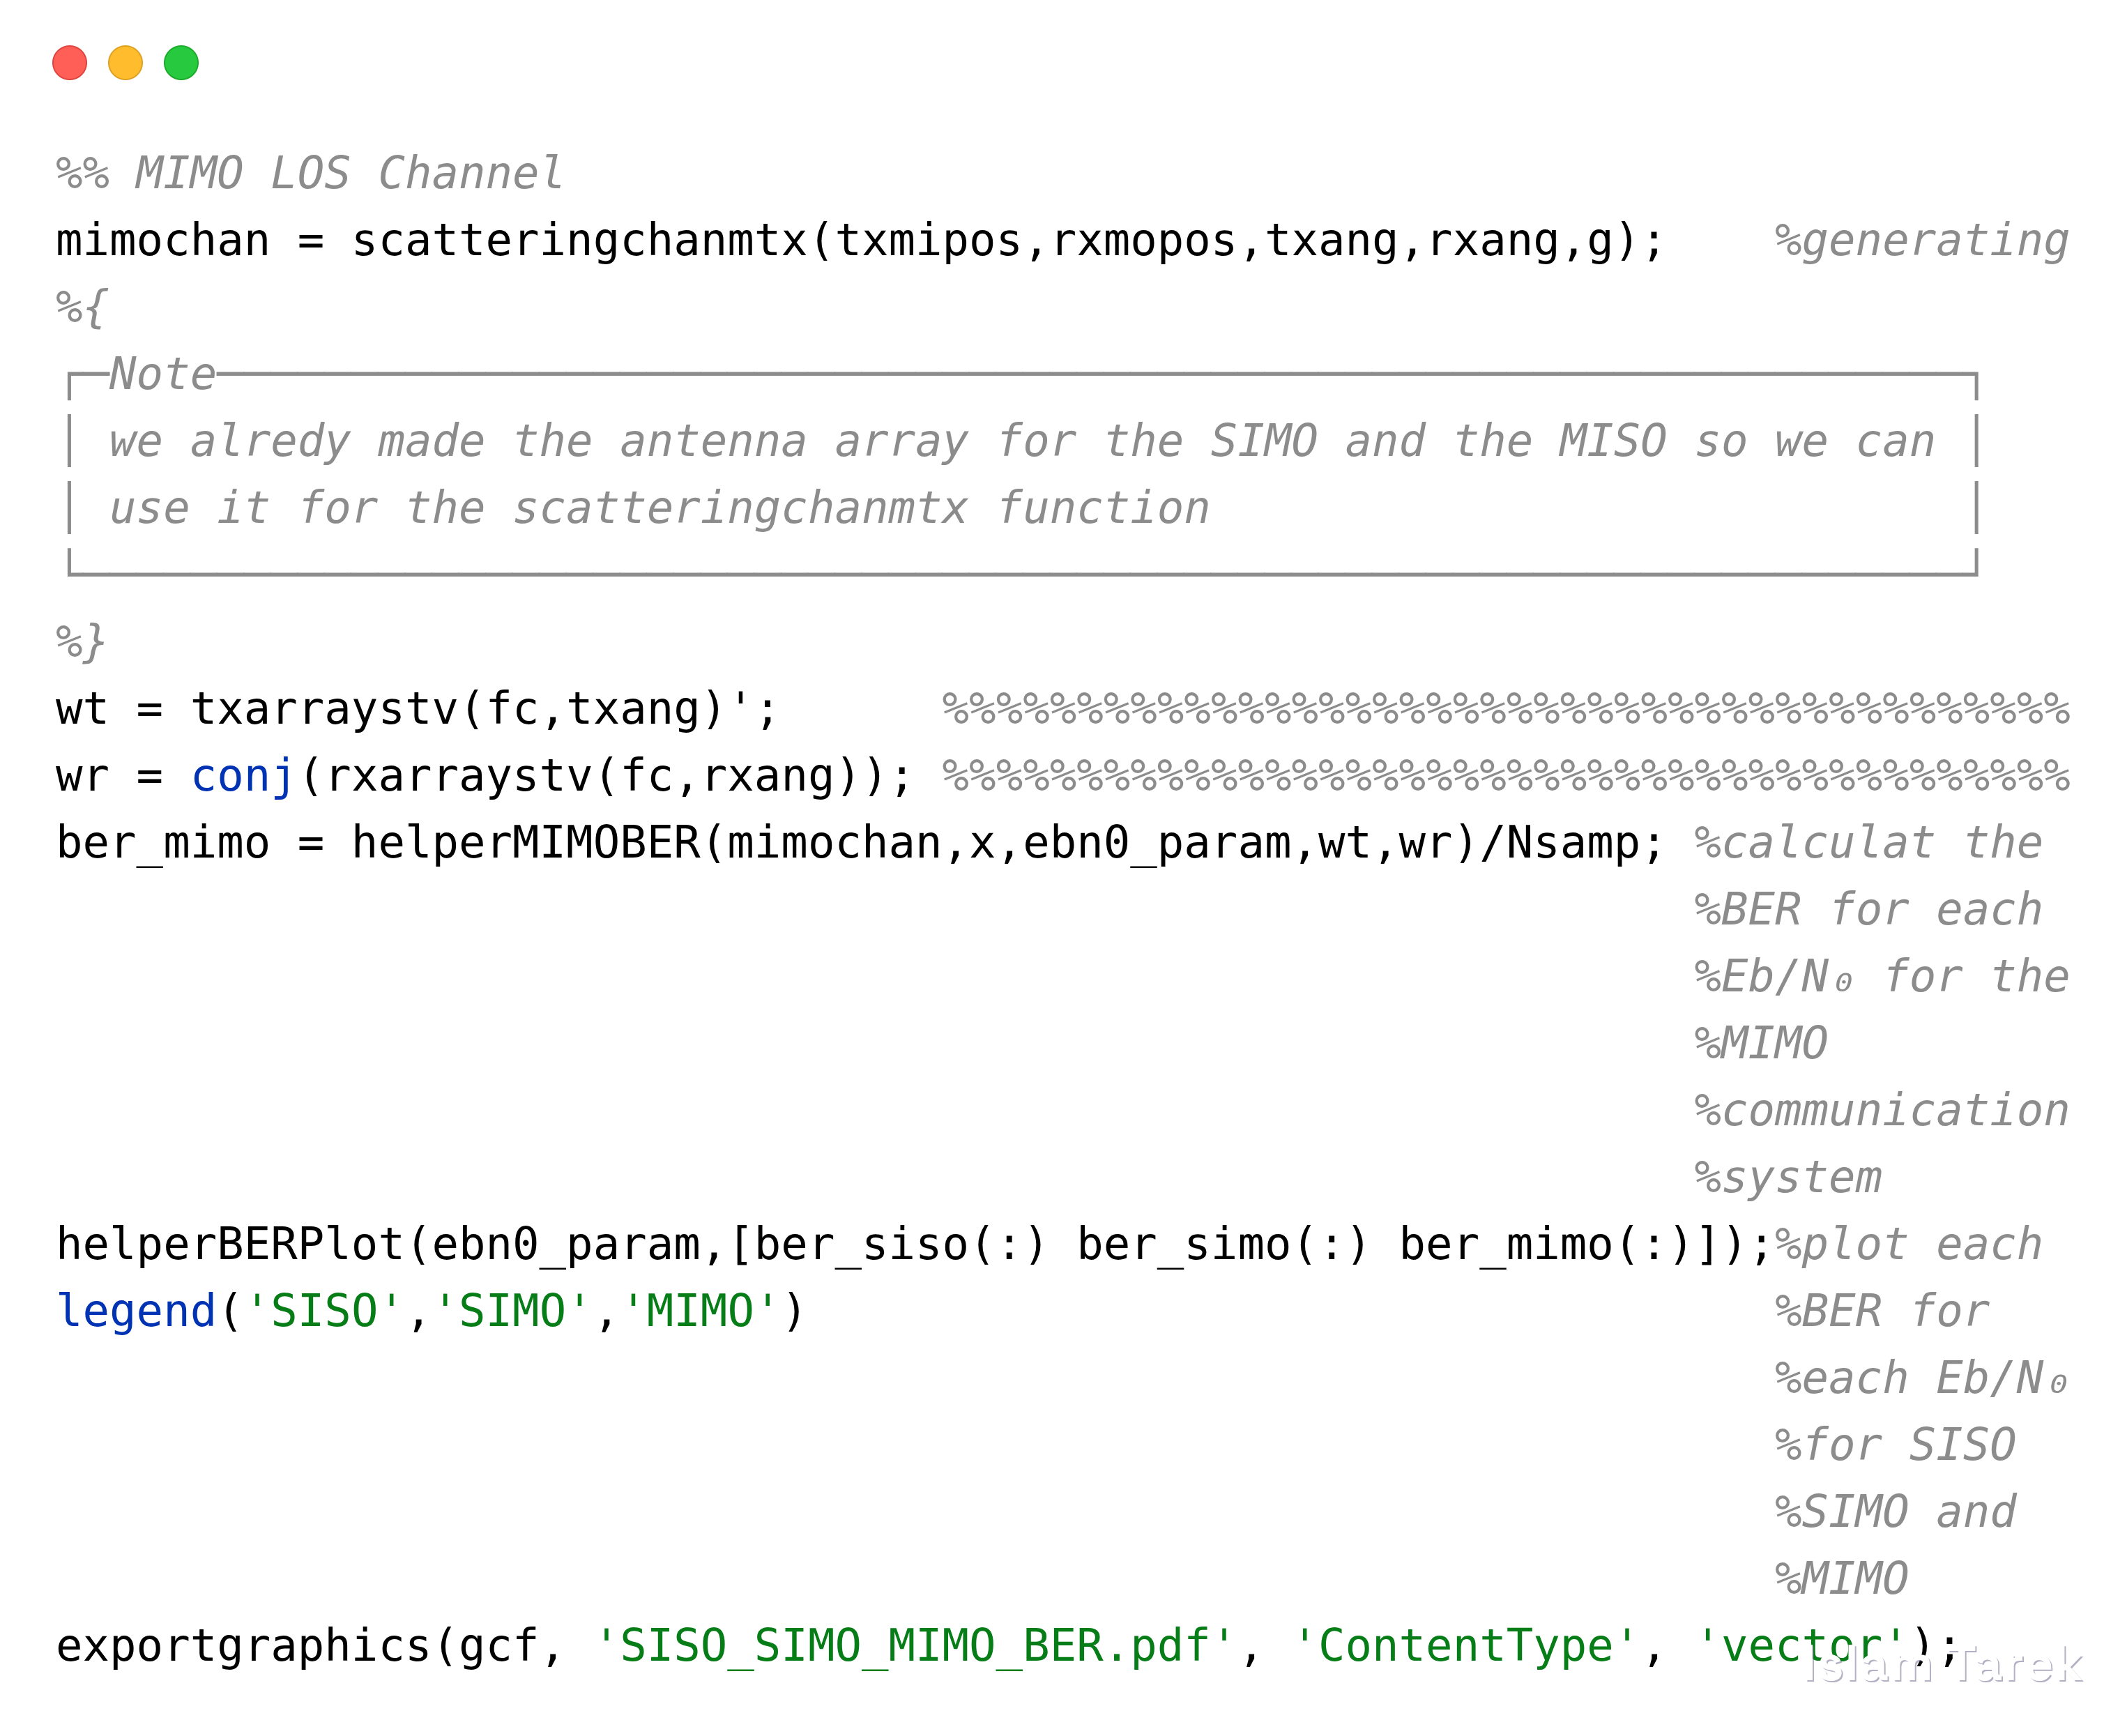
\includegraphics[width=0.7\linewidth]{figures/code5}
\end{figure}
\vfill
\restoregeometry
\chapter{Single Input Single Output Multi-path}

In real life, many problems are facing wireless communication systems. One of these problems is that the signal does not travel from the transmitter to the receiver along the LOC path only. 

\section{Delay spread}
the wave propagates and collide numerous obstacles before reaching its destination, creating a wave composed of a collection of waves with varying delays and amplitudes.

a LOC channel should have a single impulse with a delay $\tau$ in it's time-domain impulse response. in multi-path, due to scattering, we are getting more than one copy of the signal at the \Rx with different delays and amplitudes Figure[\ref{fig:delayspread}].


\begin{figure}[!h]
	\centering
	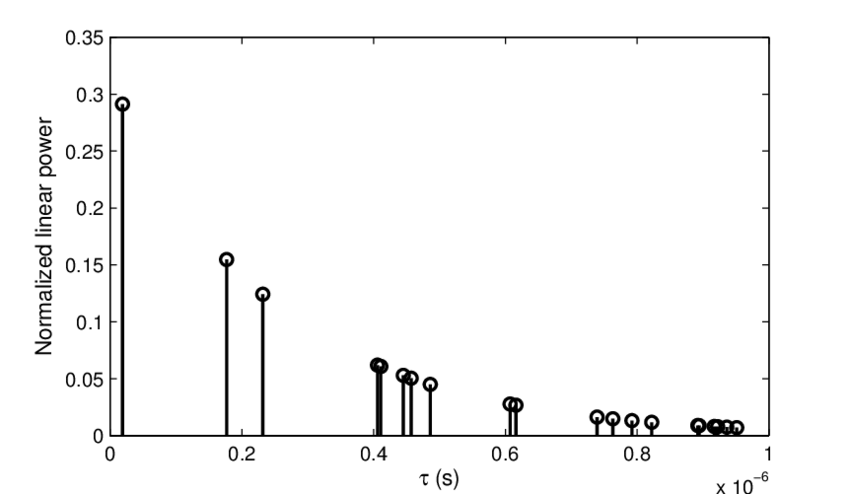
\includegraphics[width=1\linewidth]{figures/delay_spread}
	\caption{Delay Spread}
	\label{fig:delayspread}
\end{figure}

\newpage
\section{Graphical implementation}
before simulating the system we need first to be more familiar with multi-path system we will plot the multi path system we created Figure[\ref{fig:siso-multipath}].


\begin{figure}[!h]
	\centering
	\includegraphics[width=0.7\linewidth]{"figures/SISO Multipath"}
	\caption{}
	\label{fig:siso-multipath}
\end{figure}

\section{Data Generation}
in multi-path we will use a different approach of generating the data.
we will use $10^3$ frames and $10^4$ random bits for each frame.

\subsection{Simulating the system}
in this stage, we are re-simulating the system for each frame and calculating the average BER for each Eb/No.


\newpage
\section{Plotting}
after simulating the system and getting all the values needed, we are ploting the relationship between the BER and Bb/No for SISO multi-path and LOS systems to see the difference between them, and as we can see in Figure[\ref{3245}]

in multi-path graph, it's clear that it does have a higher BER than LOS one.
\begin{figure}[!h]
	\centering
	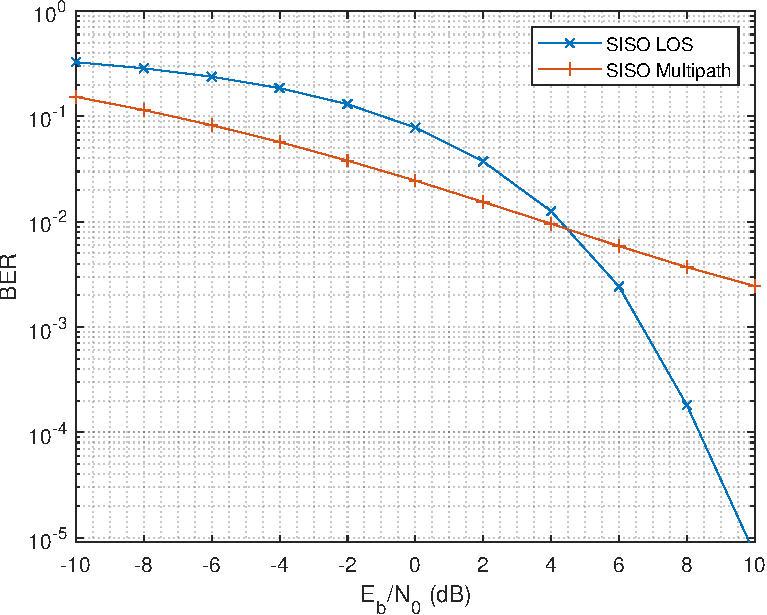
\includegraphics[width=1\linewidth]{figures/SISO_LOS_Multipath.pdf}
	\caption{SISO LOC vs Multi-path}
	\label{3245}
\end{figure}



\newgeometry{margin=0pt}
\newpage
\vfill
\begin{figure}
	\centering
	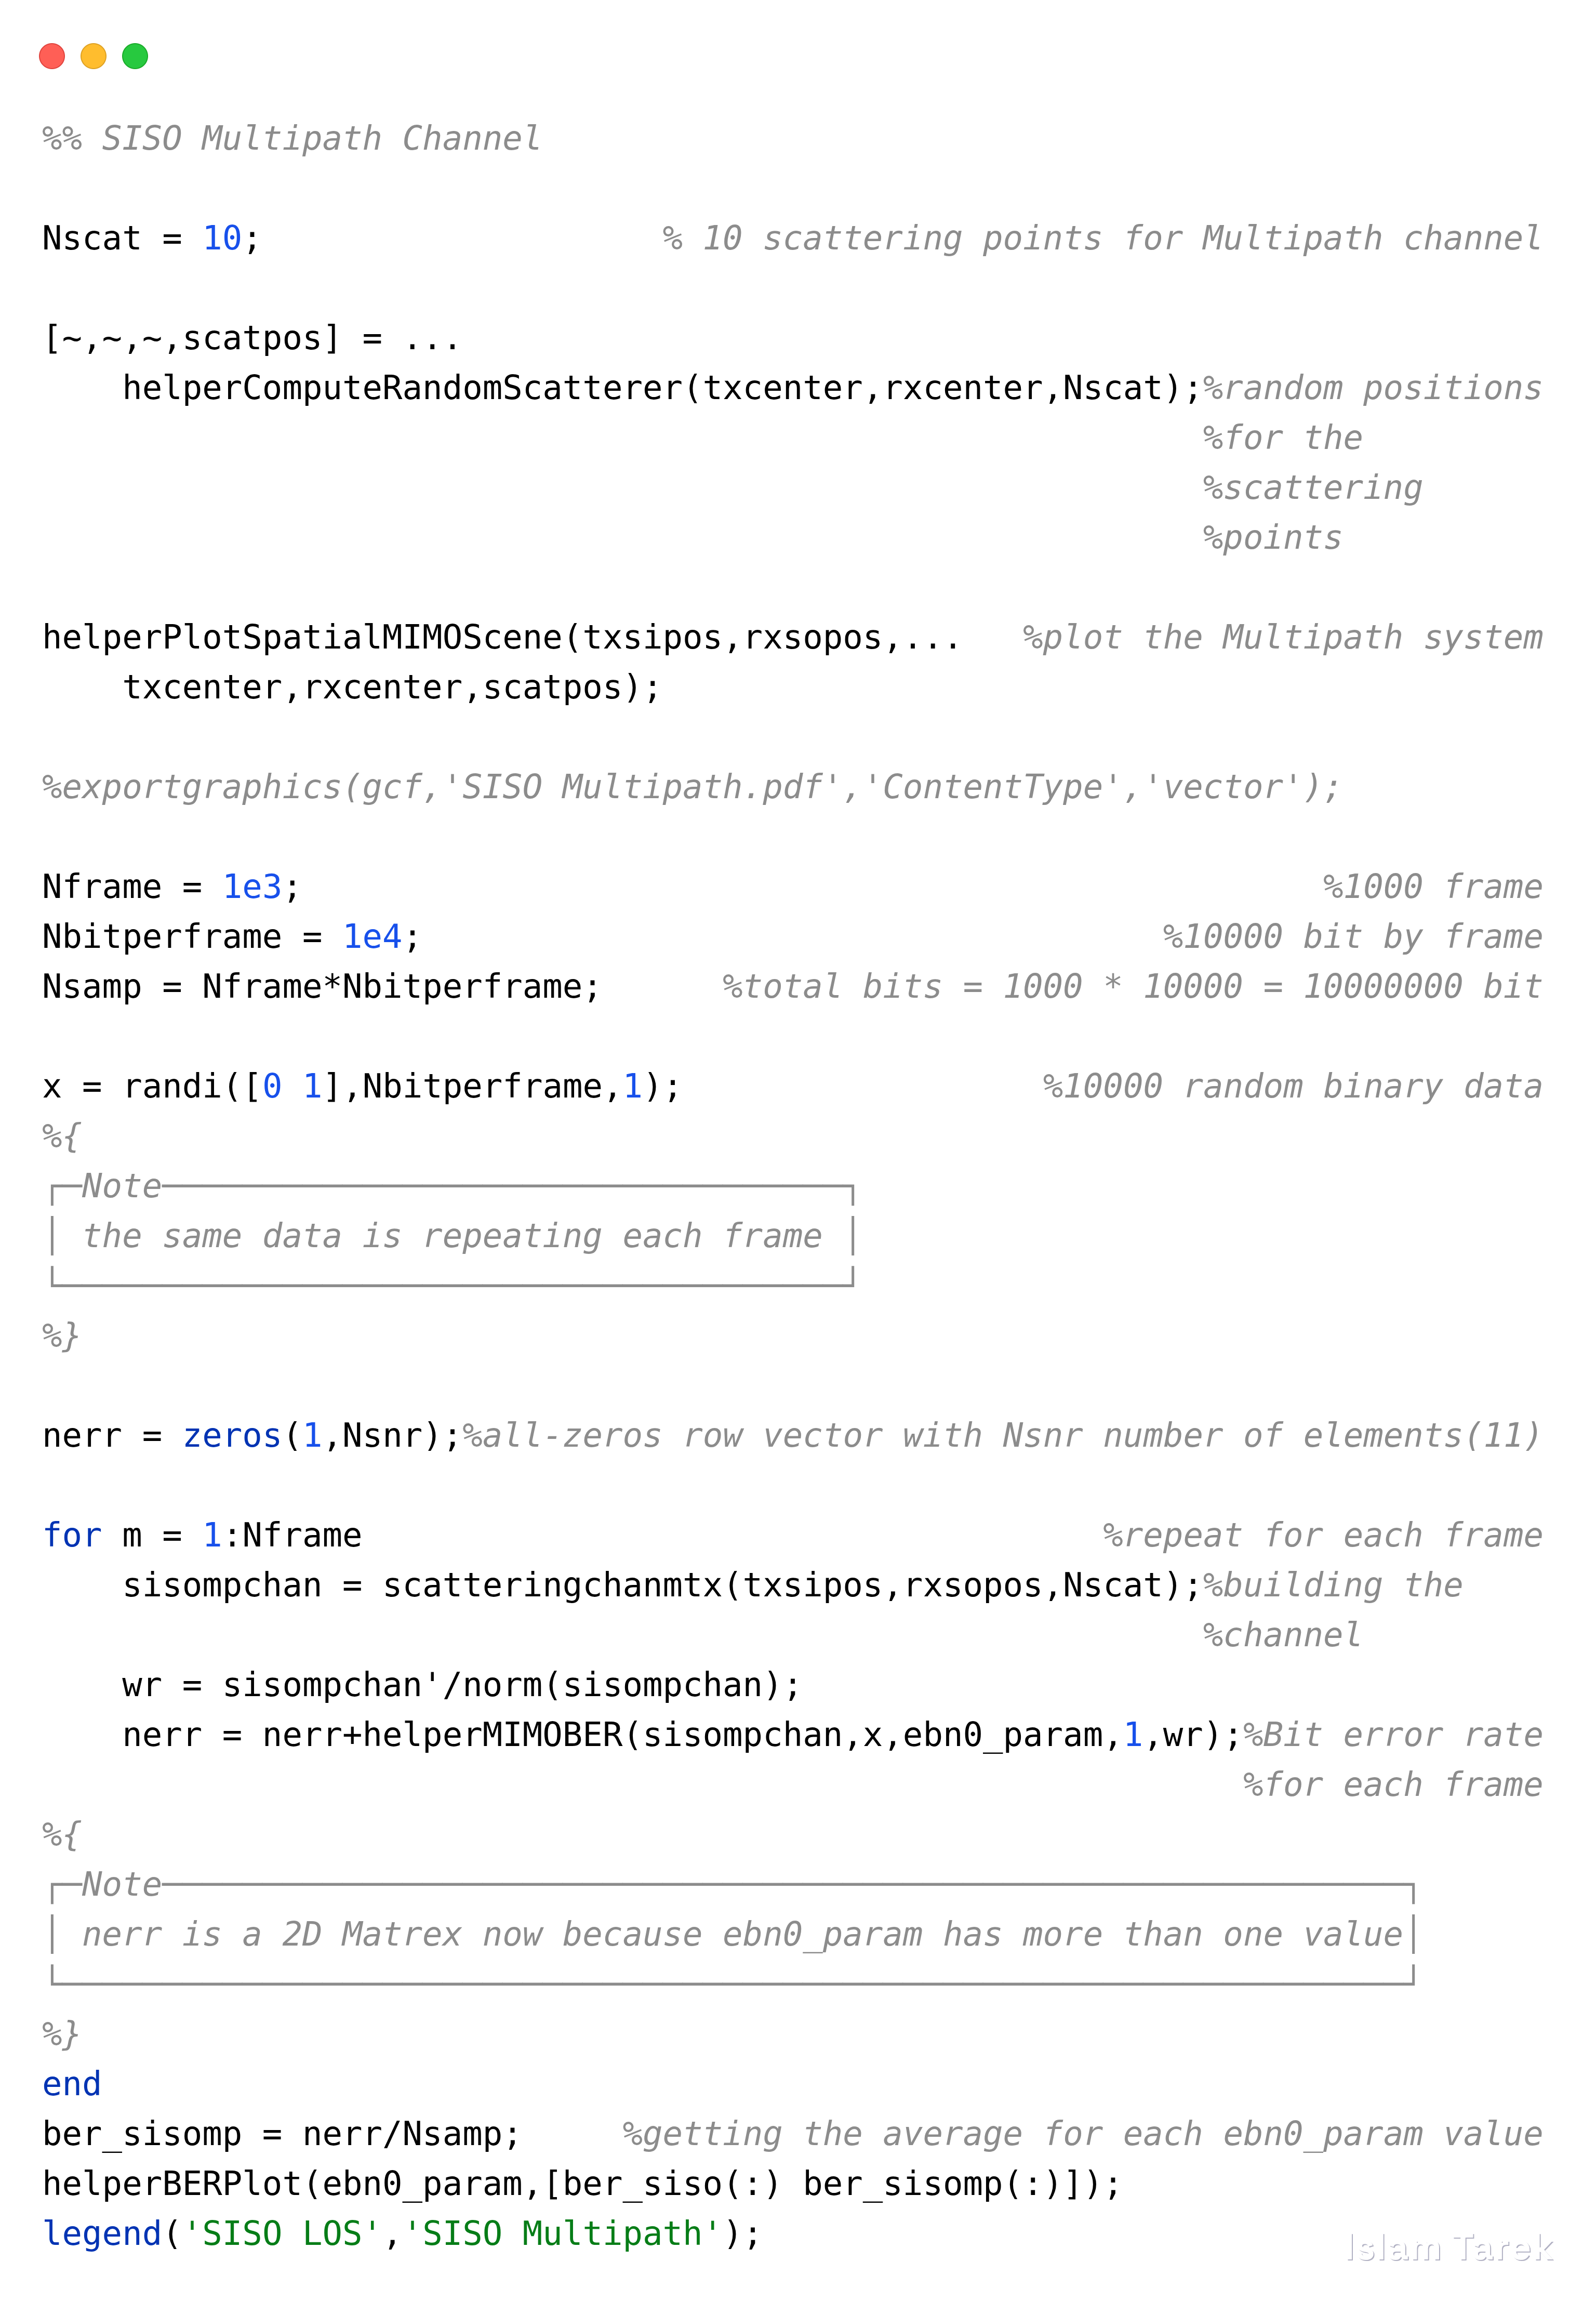
\includegraphics[width=0.7\linewidth]{figures/code6}
\end{figure}
\vfill
\restoregeometry
\chapter{SIMO and MISO Multi-path}

To avoid unnecessary repetition, we will do what we did in the previous step, except for the implementation on these two systemsز
\section{SIMO}
\begin{figure}[!h]
	\centering
	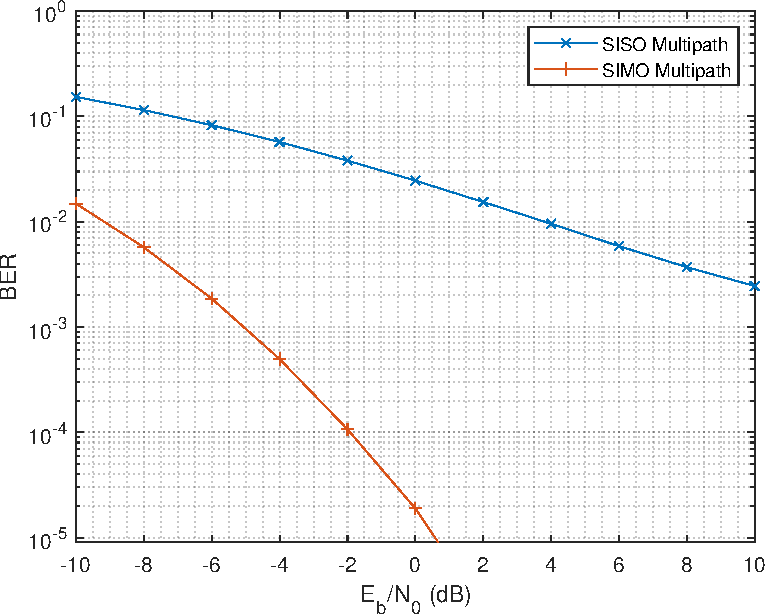
\includegraphics[width=1\linewidth]{figures/SISO_SIMO Multipath.pdf}
	\caption{SISO LOC vs Multi-path}
	\label{32545}
\end{figure}
as we can see in Figure[\ref{32545}], for multi-path SIMO, the BER is smaller than multi-path SIMO , and that's because of the spatial diversity and also because the signal is forming in a beam that is more focusing in one direction.
\section{MISO}
\begin{figure}[!h]
	\centering
	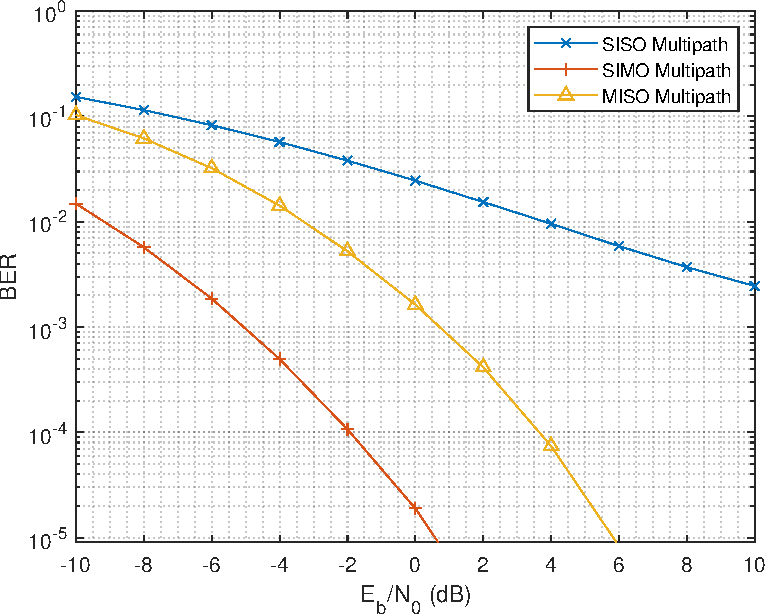
\includegraphics[width=1\linewidth]{figures/SISO_SIMO_MISO Multipath.pdf}
	\caption{SISO LOC vs Multi-path}
	\label{3575}
\end{figure}

and for multi-path MISO, the antenna in the \Tx is less directed towards the \Rx than the \Rx was in the SIMO system, the beam is less saturated and the destructive fading is more than it was in this case at the \Rx, so we are seeing a better BER for SIMO here Figure[\ref{3575}].

\newgeometry{margin=0pt}
\newpage
\vfill
\begin{figure}
	\centering
	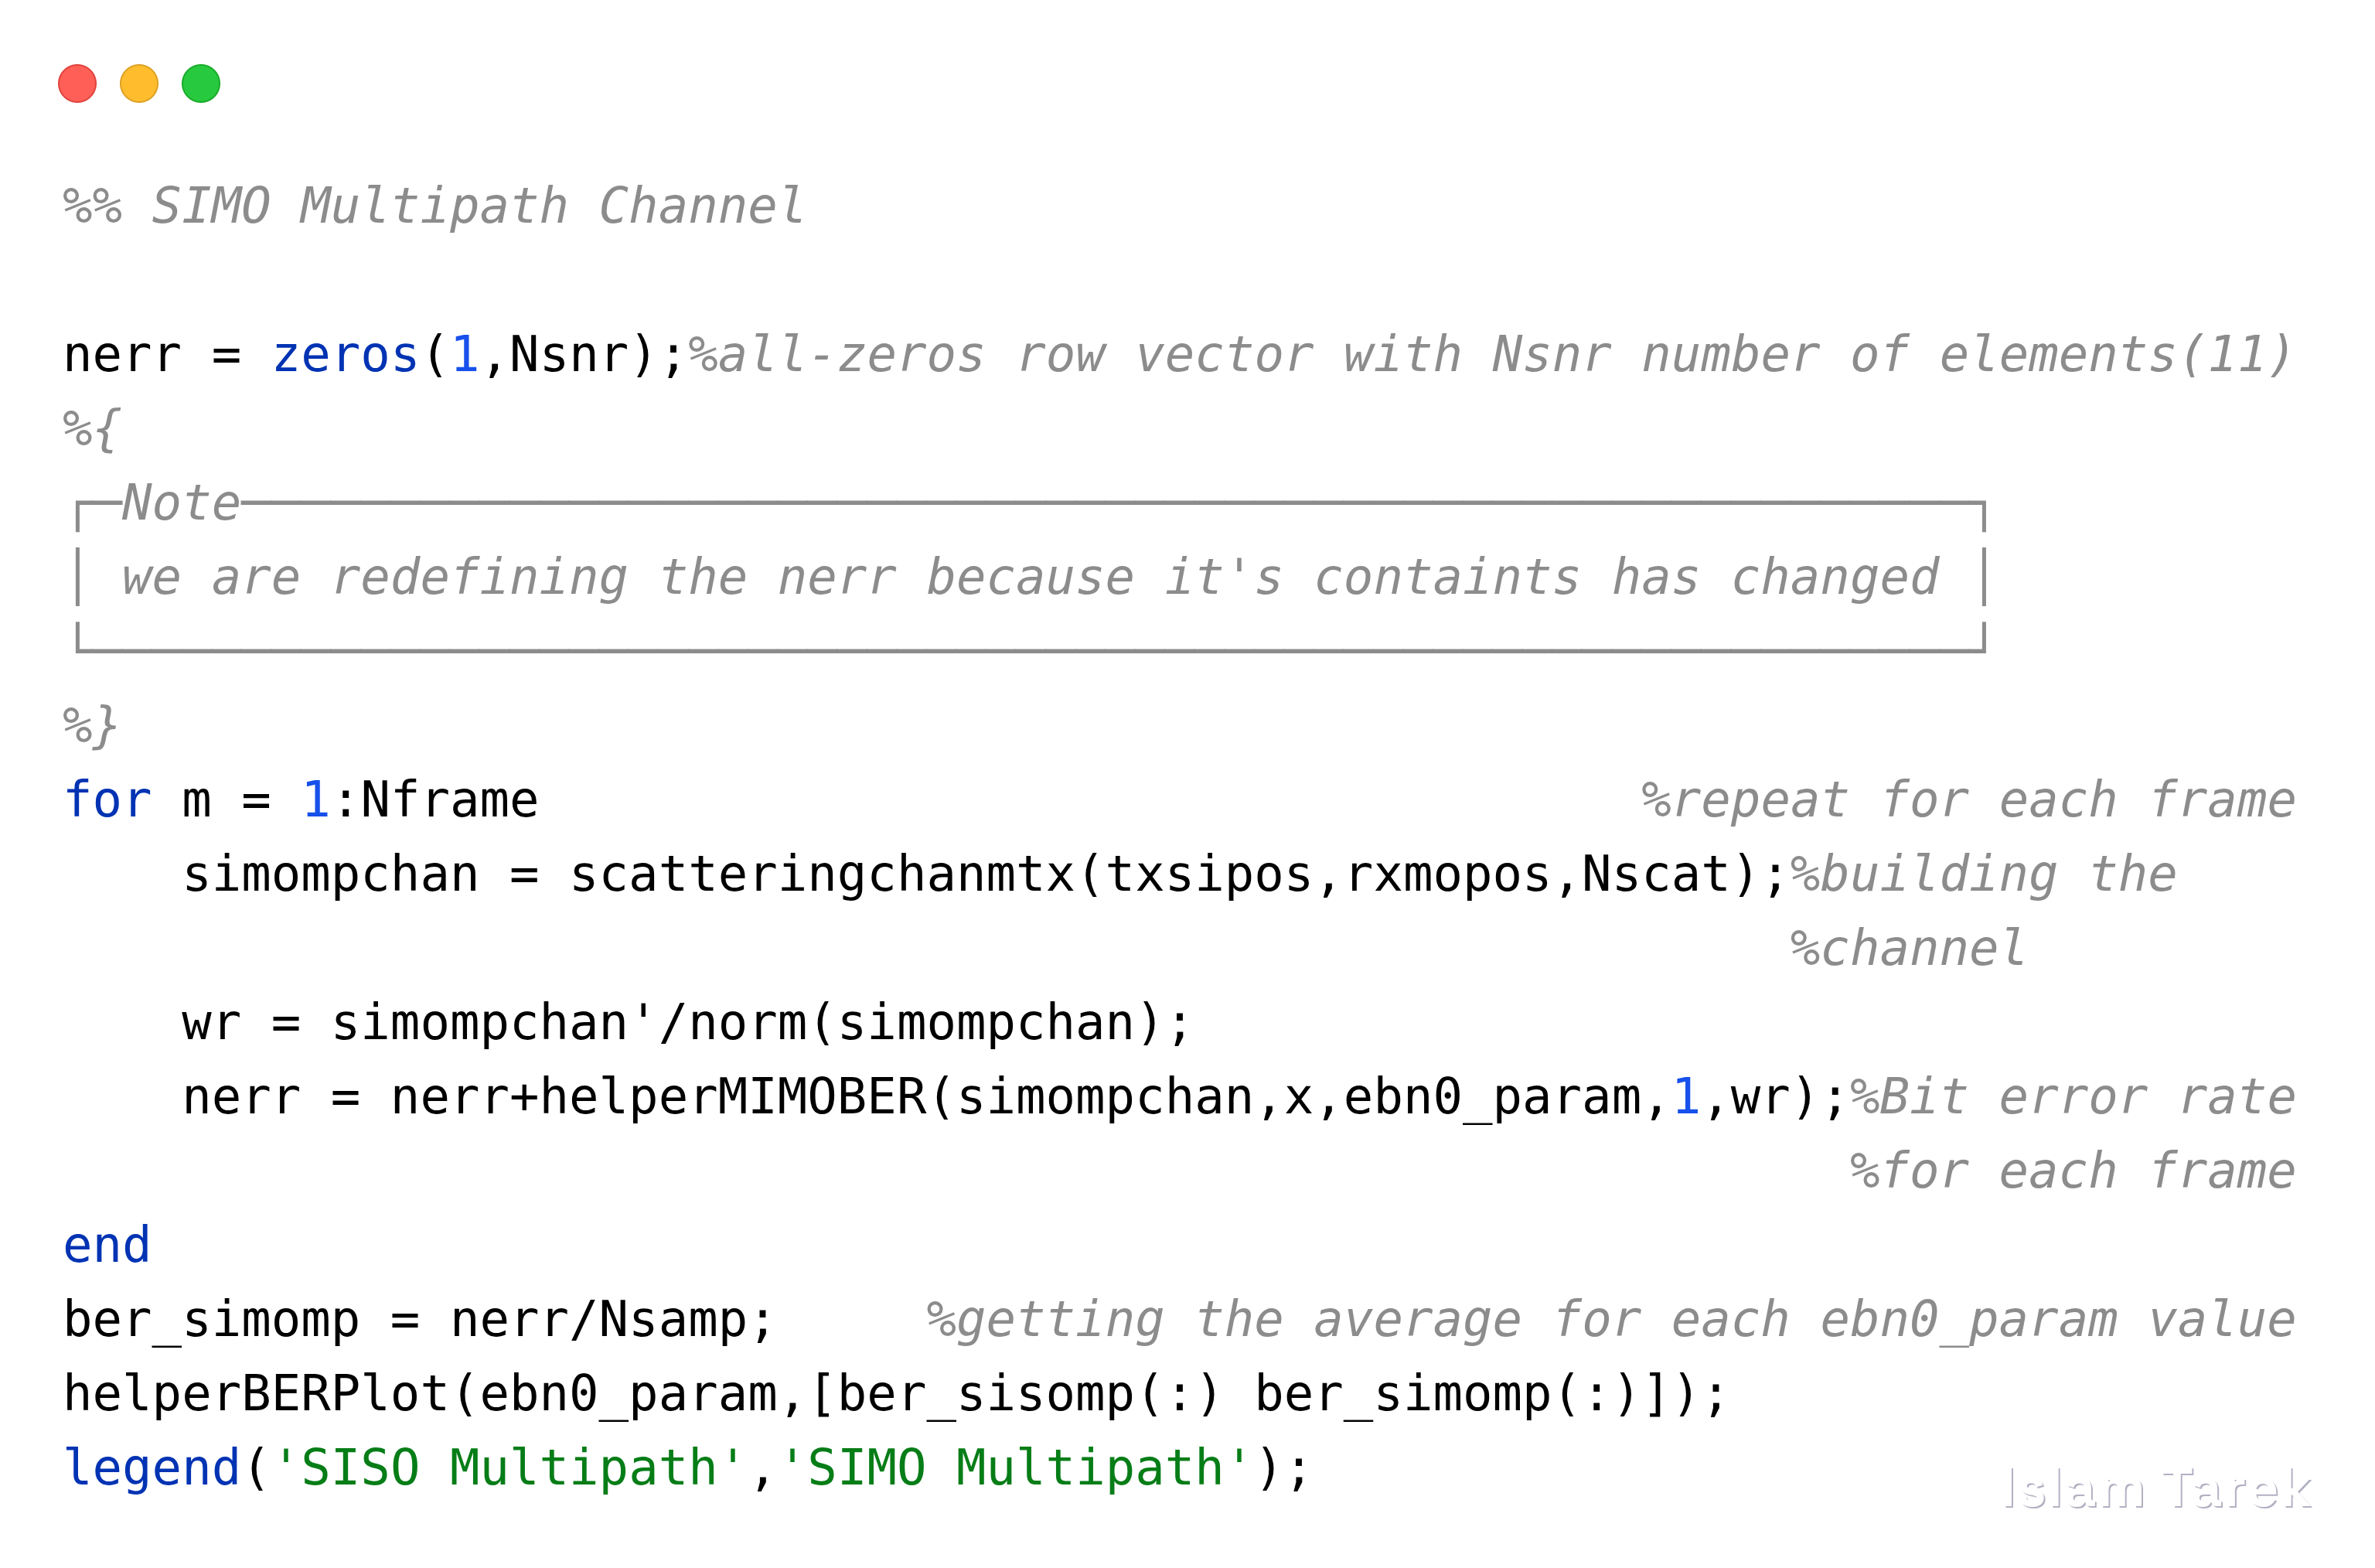
\includegraphics[width=0.7\linewidth]{figures/code7}
\end{figure}
\begin{figure}
	\centering
	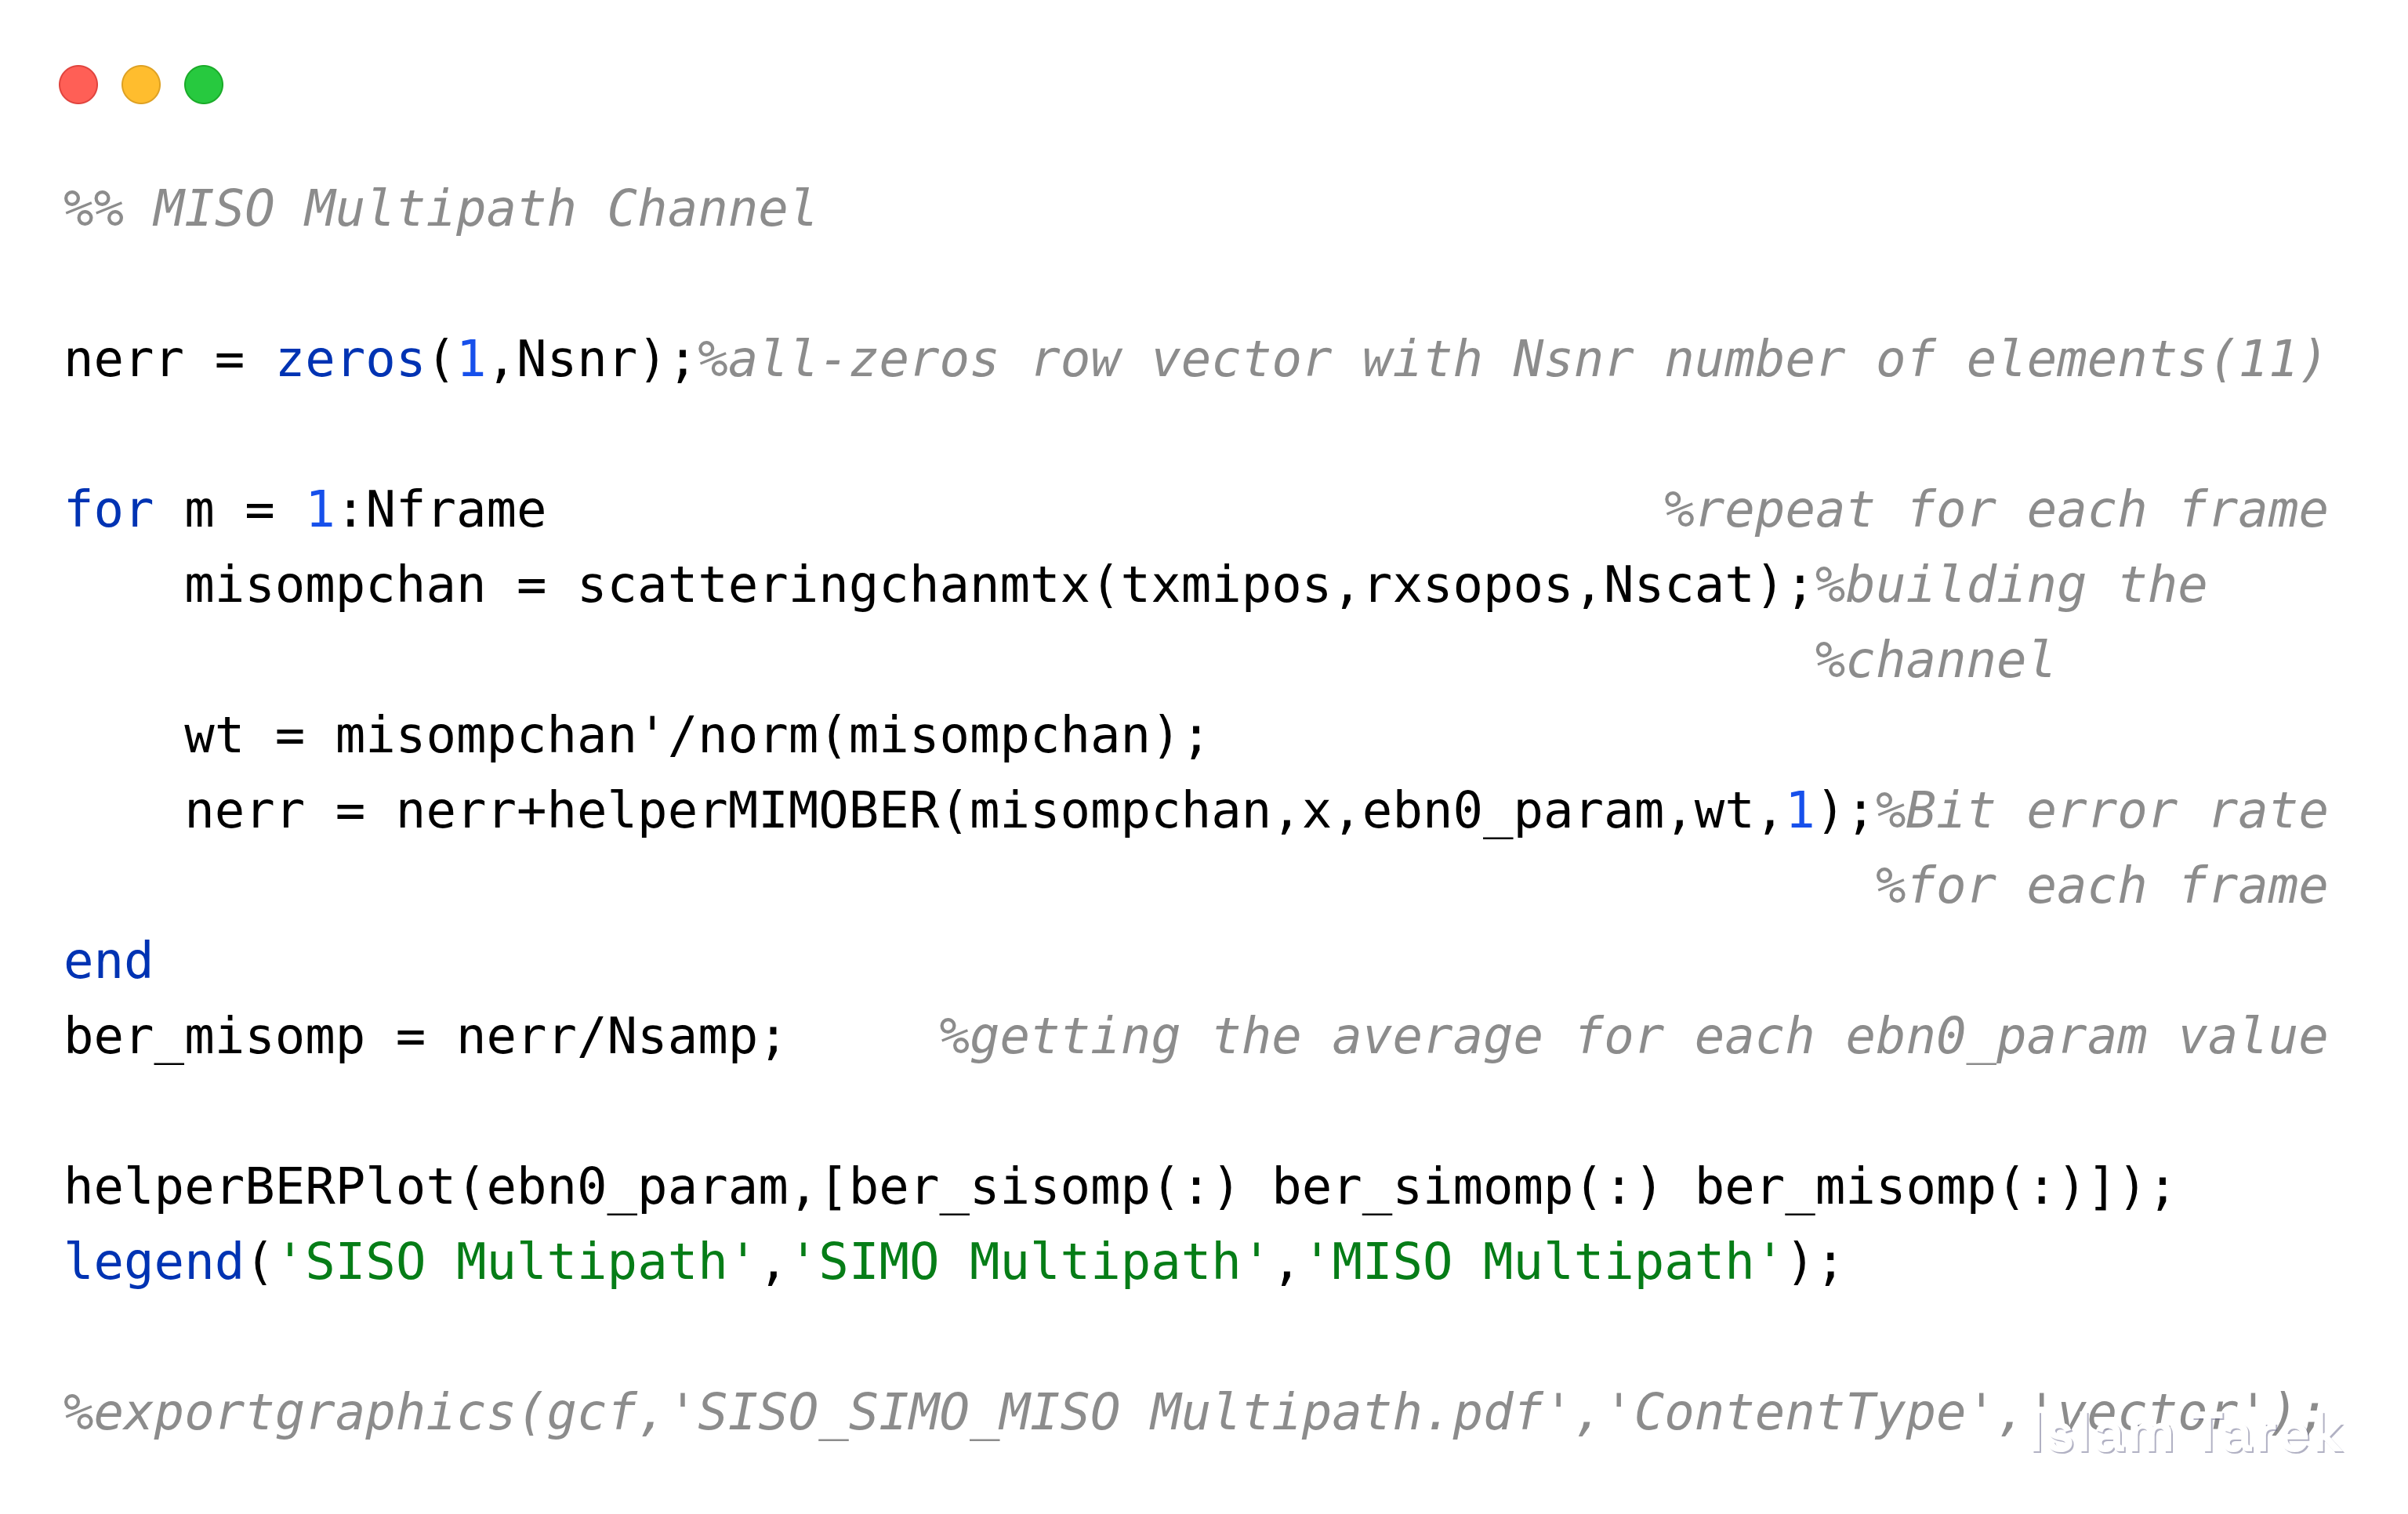
\includegraphics[width=0.7\linewidth]{figures/code8}
\end{figure}
\vfill
\restoregeometry
\chapter{Multiple Input Multiple Output Multi-path}

we will do as we did in SISO here.
\begin{enumerate}
	\item graphical representation of the system
	\item bulding the scattering maxrex for each frame and calculating the BER for each Eb/No
	\item plotting the relationship between BER and Eb/No for the MIMO system.
\end{enumerate}

\section{Graphical implementation}
before simulating the system we need first to be more familiar with multi-path system we will plot the multi path system we created Figure[\ref{fig:MIMO-multipath}].


\begin{figure}[!h]
	\centering
	
\includegraphics[width=0.7\linewidth]{"figures/MIMO Multipath.pdf"}
	\caption{}
	\label{fig:MIMO-multipath}
\end{figure}


\subsection{Simulating the system}
in this stage, we are re-simulating the system for each frame and calculating the average BER for each Eb/No.

\section{Plotting}
after simulating the system and getting all the values needed, we are ploting the relationship between the BER and Bb/No for SISO, SIMO, MIMO multi-path systems to see the diffrence between them Figure[\ref{32345}].

and as we can see, the BER in MIMO is not only lesser than the BER in SIMO, but also has faster decline.

\begin{figure}[!h]
	\centering
	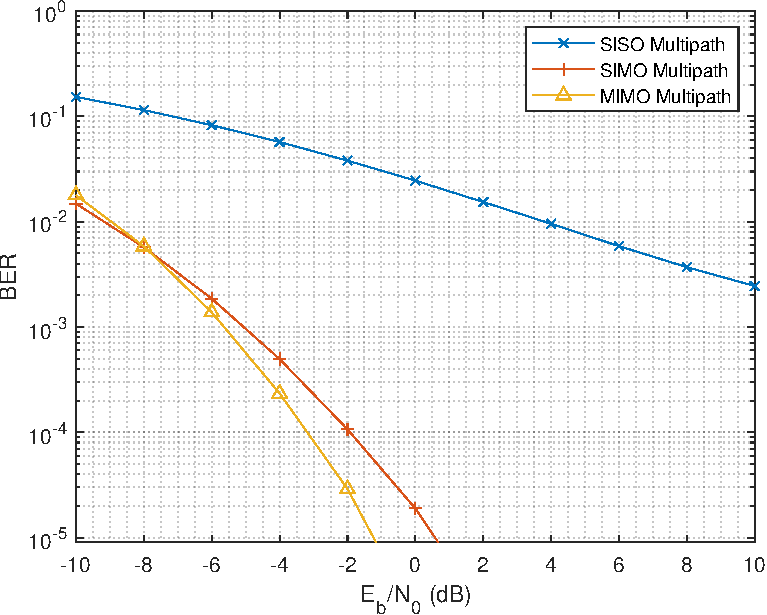
\includegraphics[width=1\linewidth]{figures/SISO_SIMO_MIMO Multipath.pdf}
	\caption{SISO LOC vs Multi-path}
	\label{32345}
\end{figure}



\newgeometry{margin=0pt}
\newpage
\vfill
\begin{figure}
	\centering
	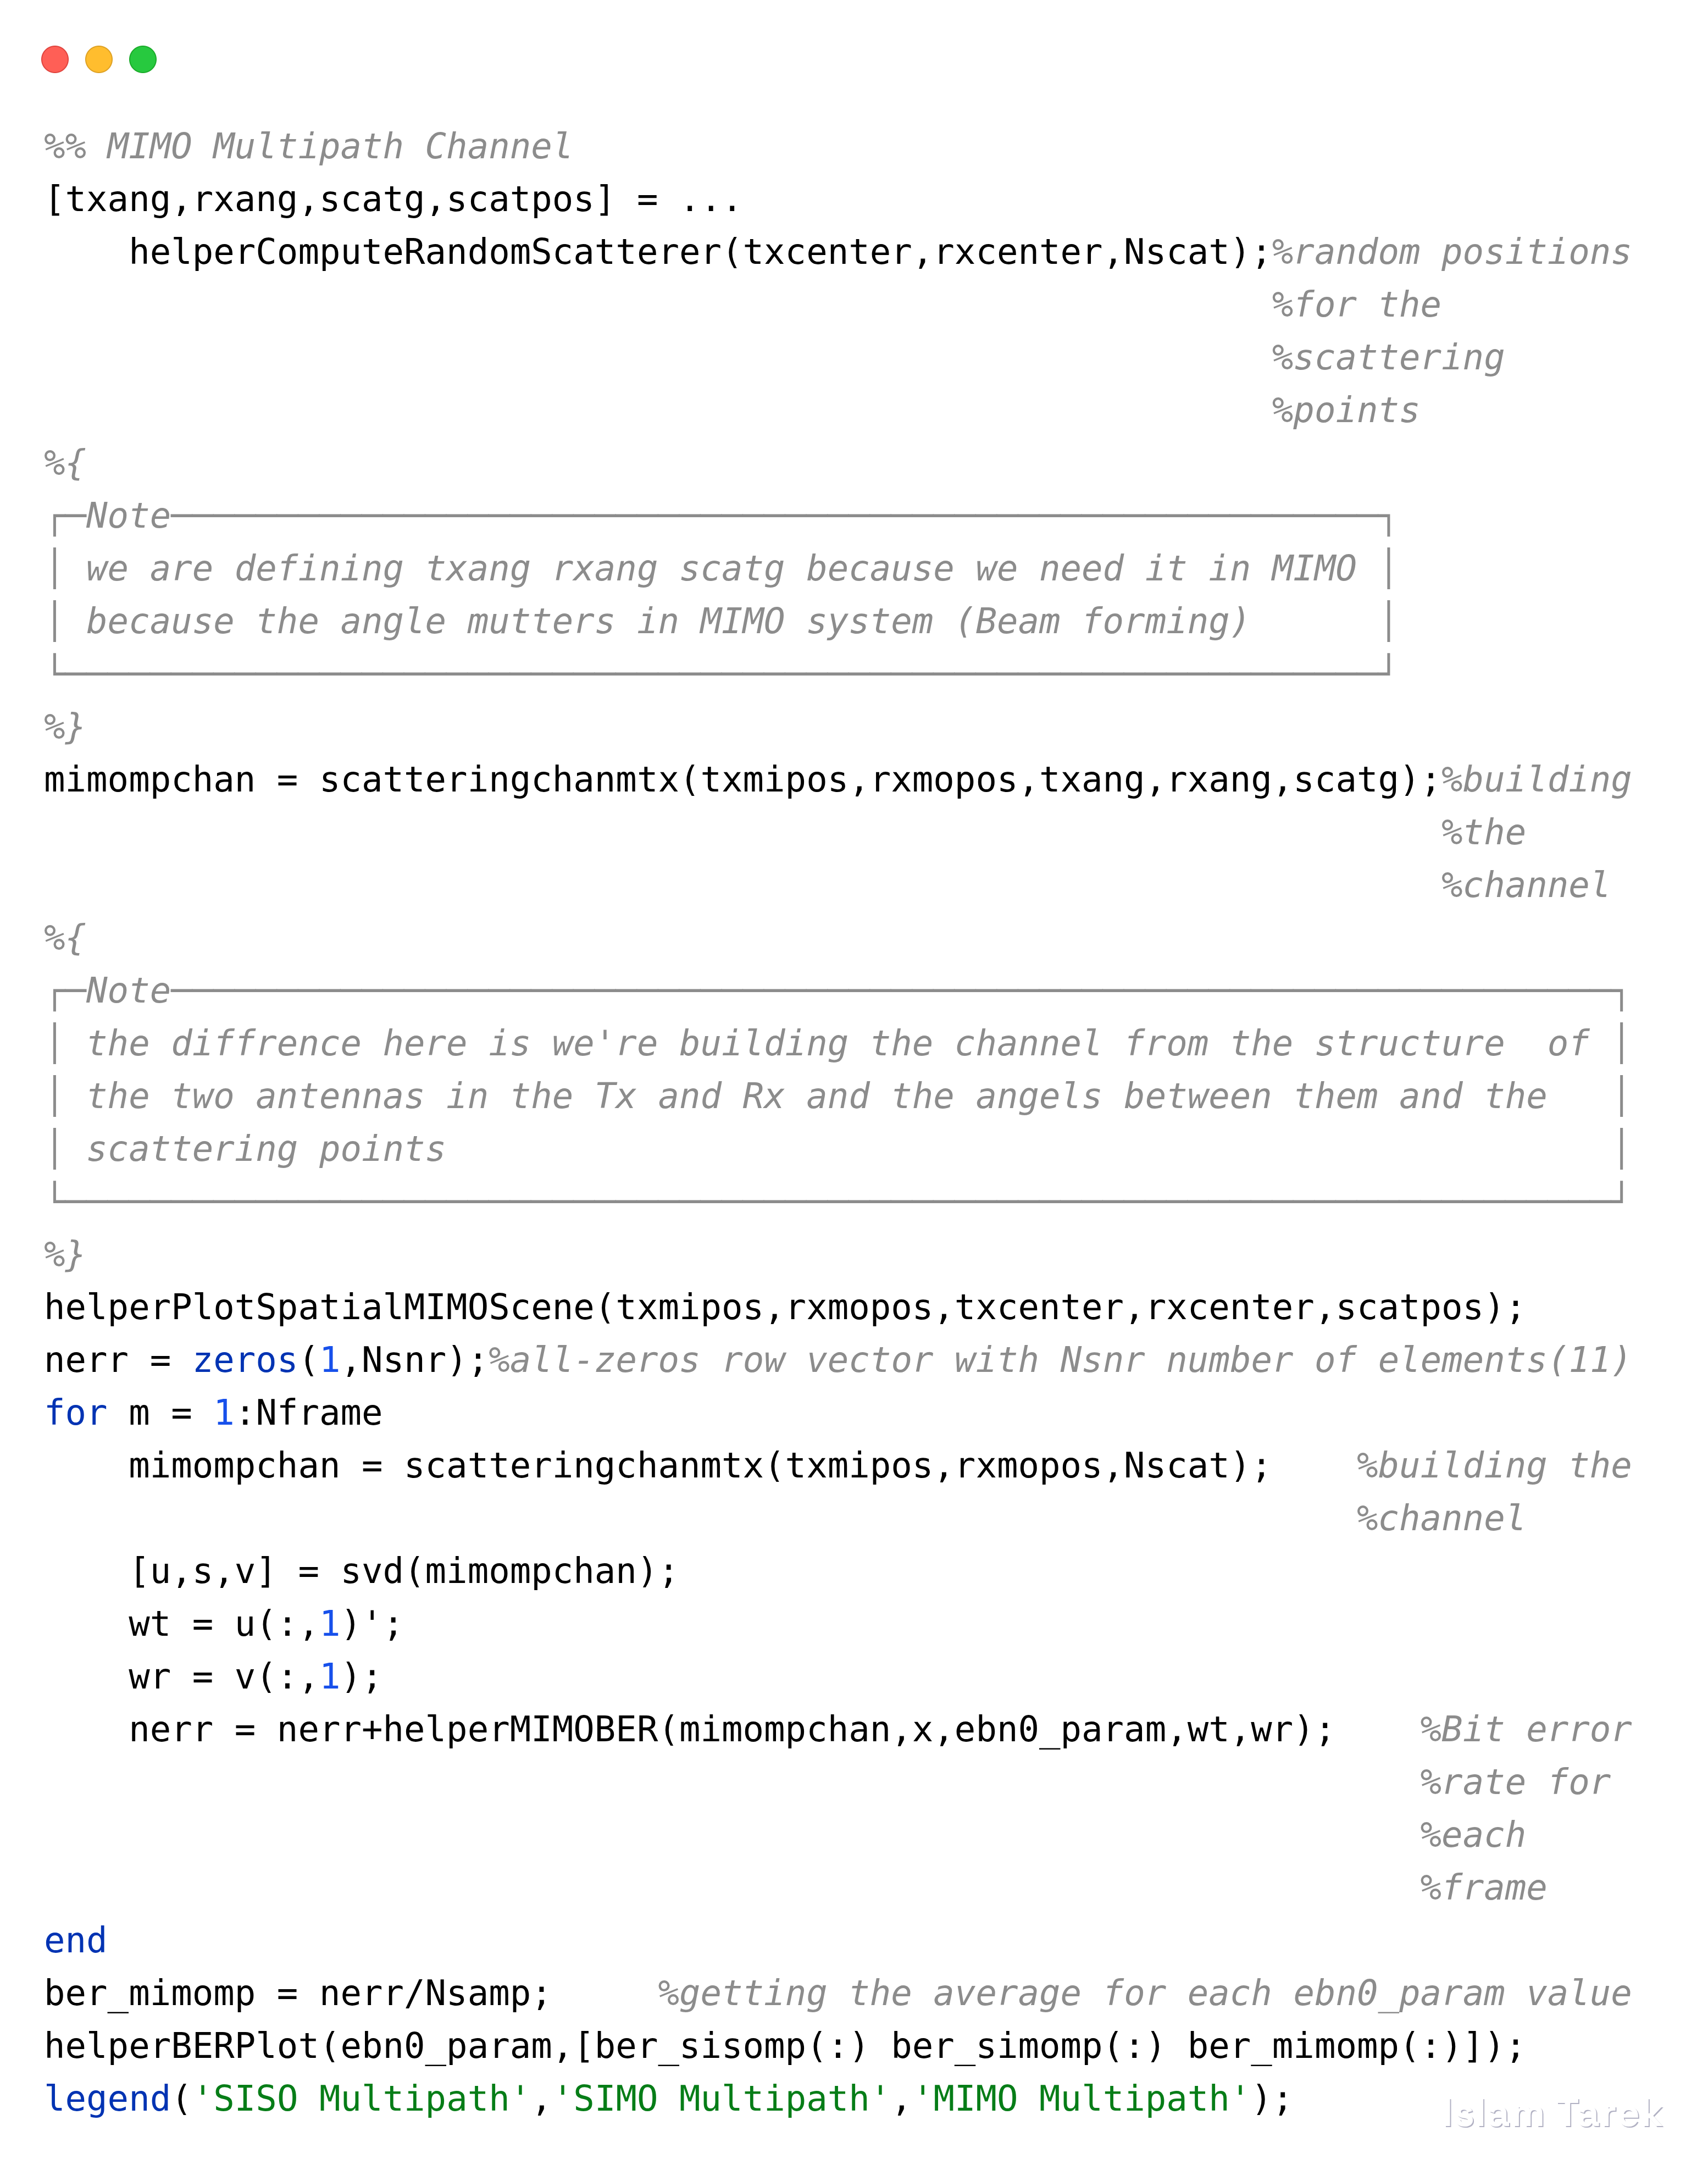
\includegraphics[width=0.7\linewidth]{figures/code9}
\end{figure}
\vfill
\restoregeometry

%\input{mainmatter/conclusion}

%% Prevent urls running into margins in bibliography
\setcounter{biburlnumpenalty}{7000}
\setcounter{biburllcpenalty}{7000}
\setcounter{biburlucpenalty}{7000}

%% Add bibliography
\printbibliography[heading=bibintoc,title=References]

%% ----------------------------------------------------------------------
%%    Appendix (Letters for chapters)
%% ----------------------------------------------------------------------

\appendix

\chapter{Full MATLAB Code}
%\label{chapter:title}


\newgeometry{margin=0pt}
\newpage
\begin{figure}
	\centering
	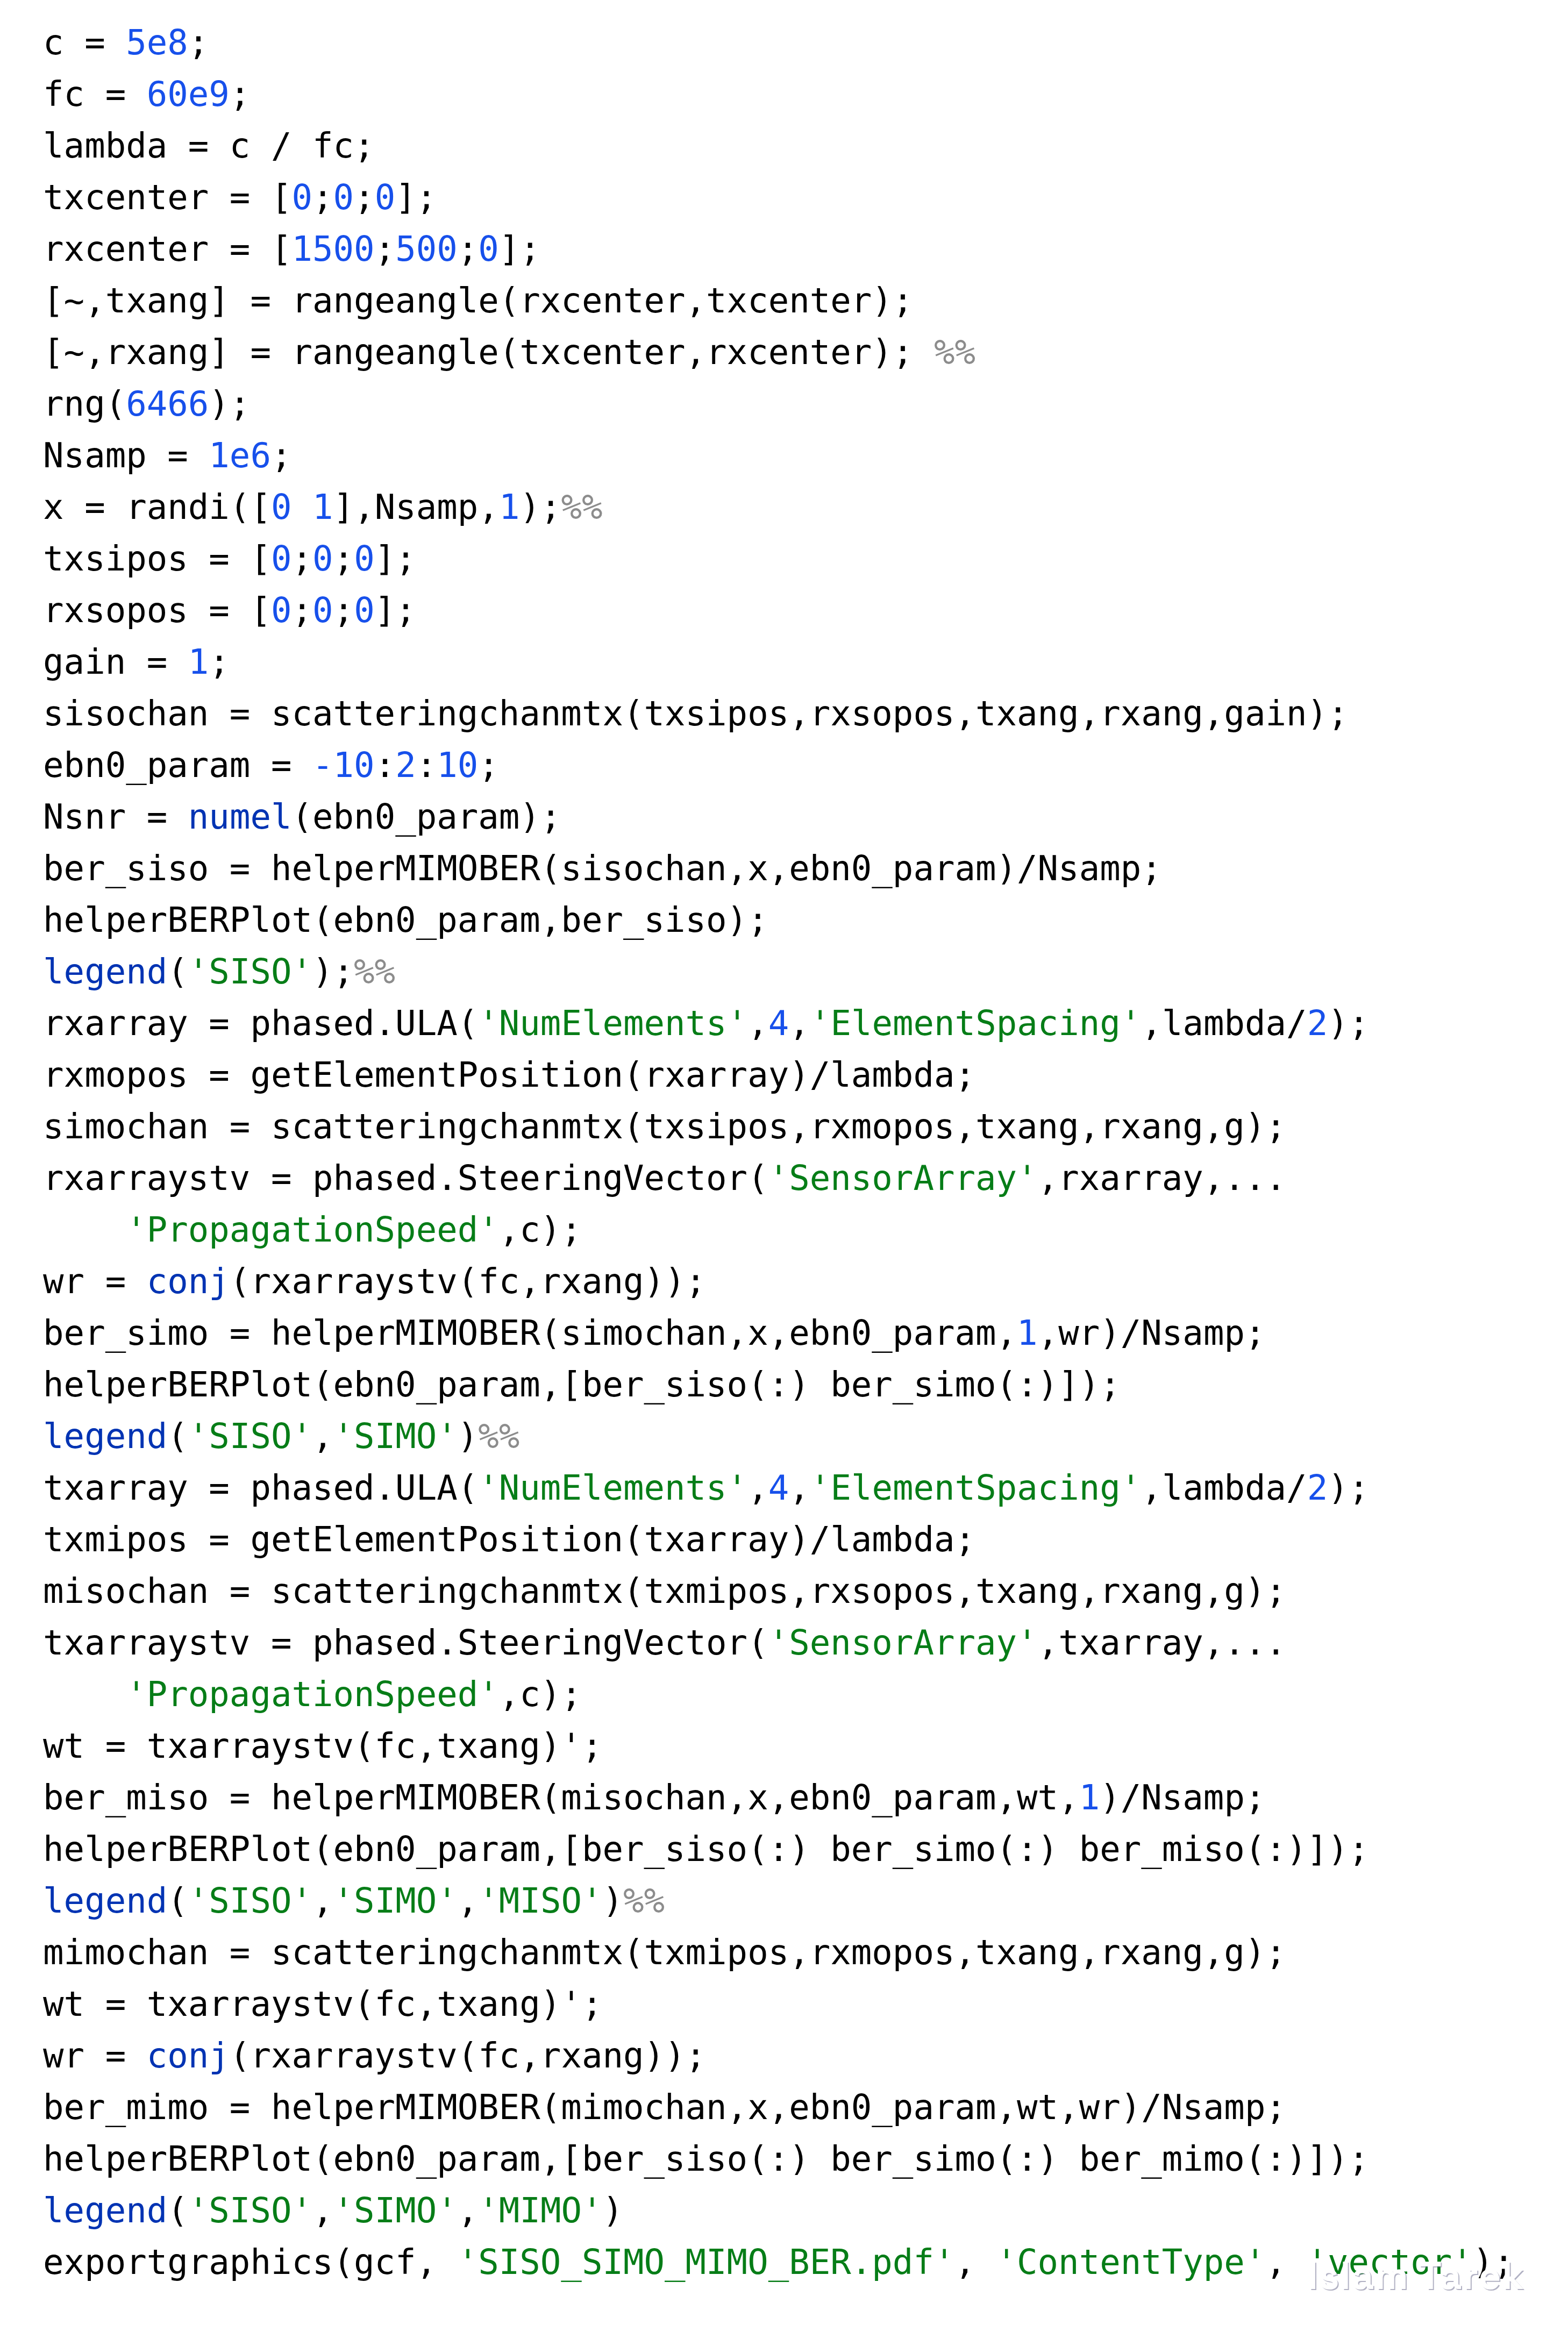
\includegraphics[width=0.8\linewidth]{figures/fullcode2}
\end{figure}
\restoregeometry
\newpage
\newgeometry{margin=0pt}
\newpage
\begin{figure}
	\centering
	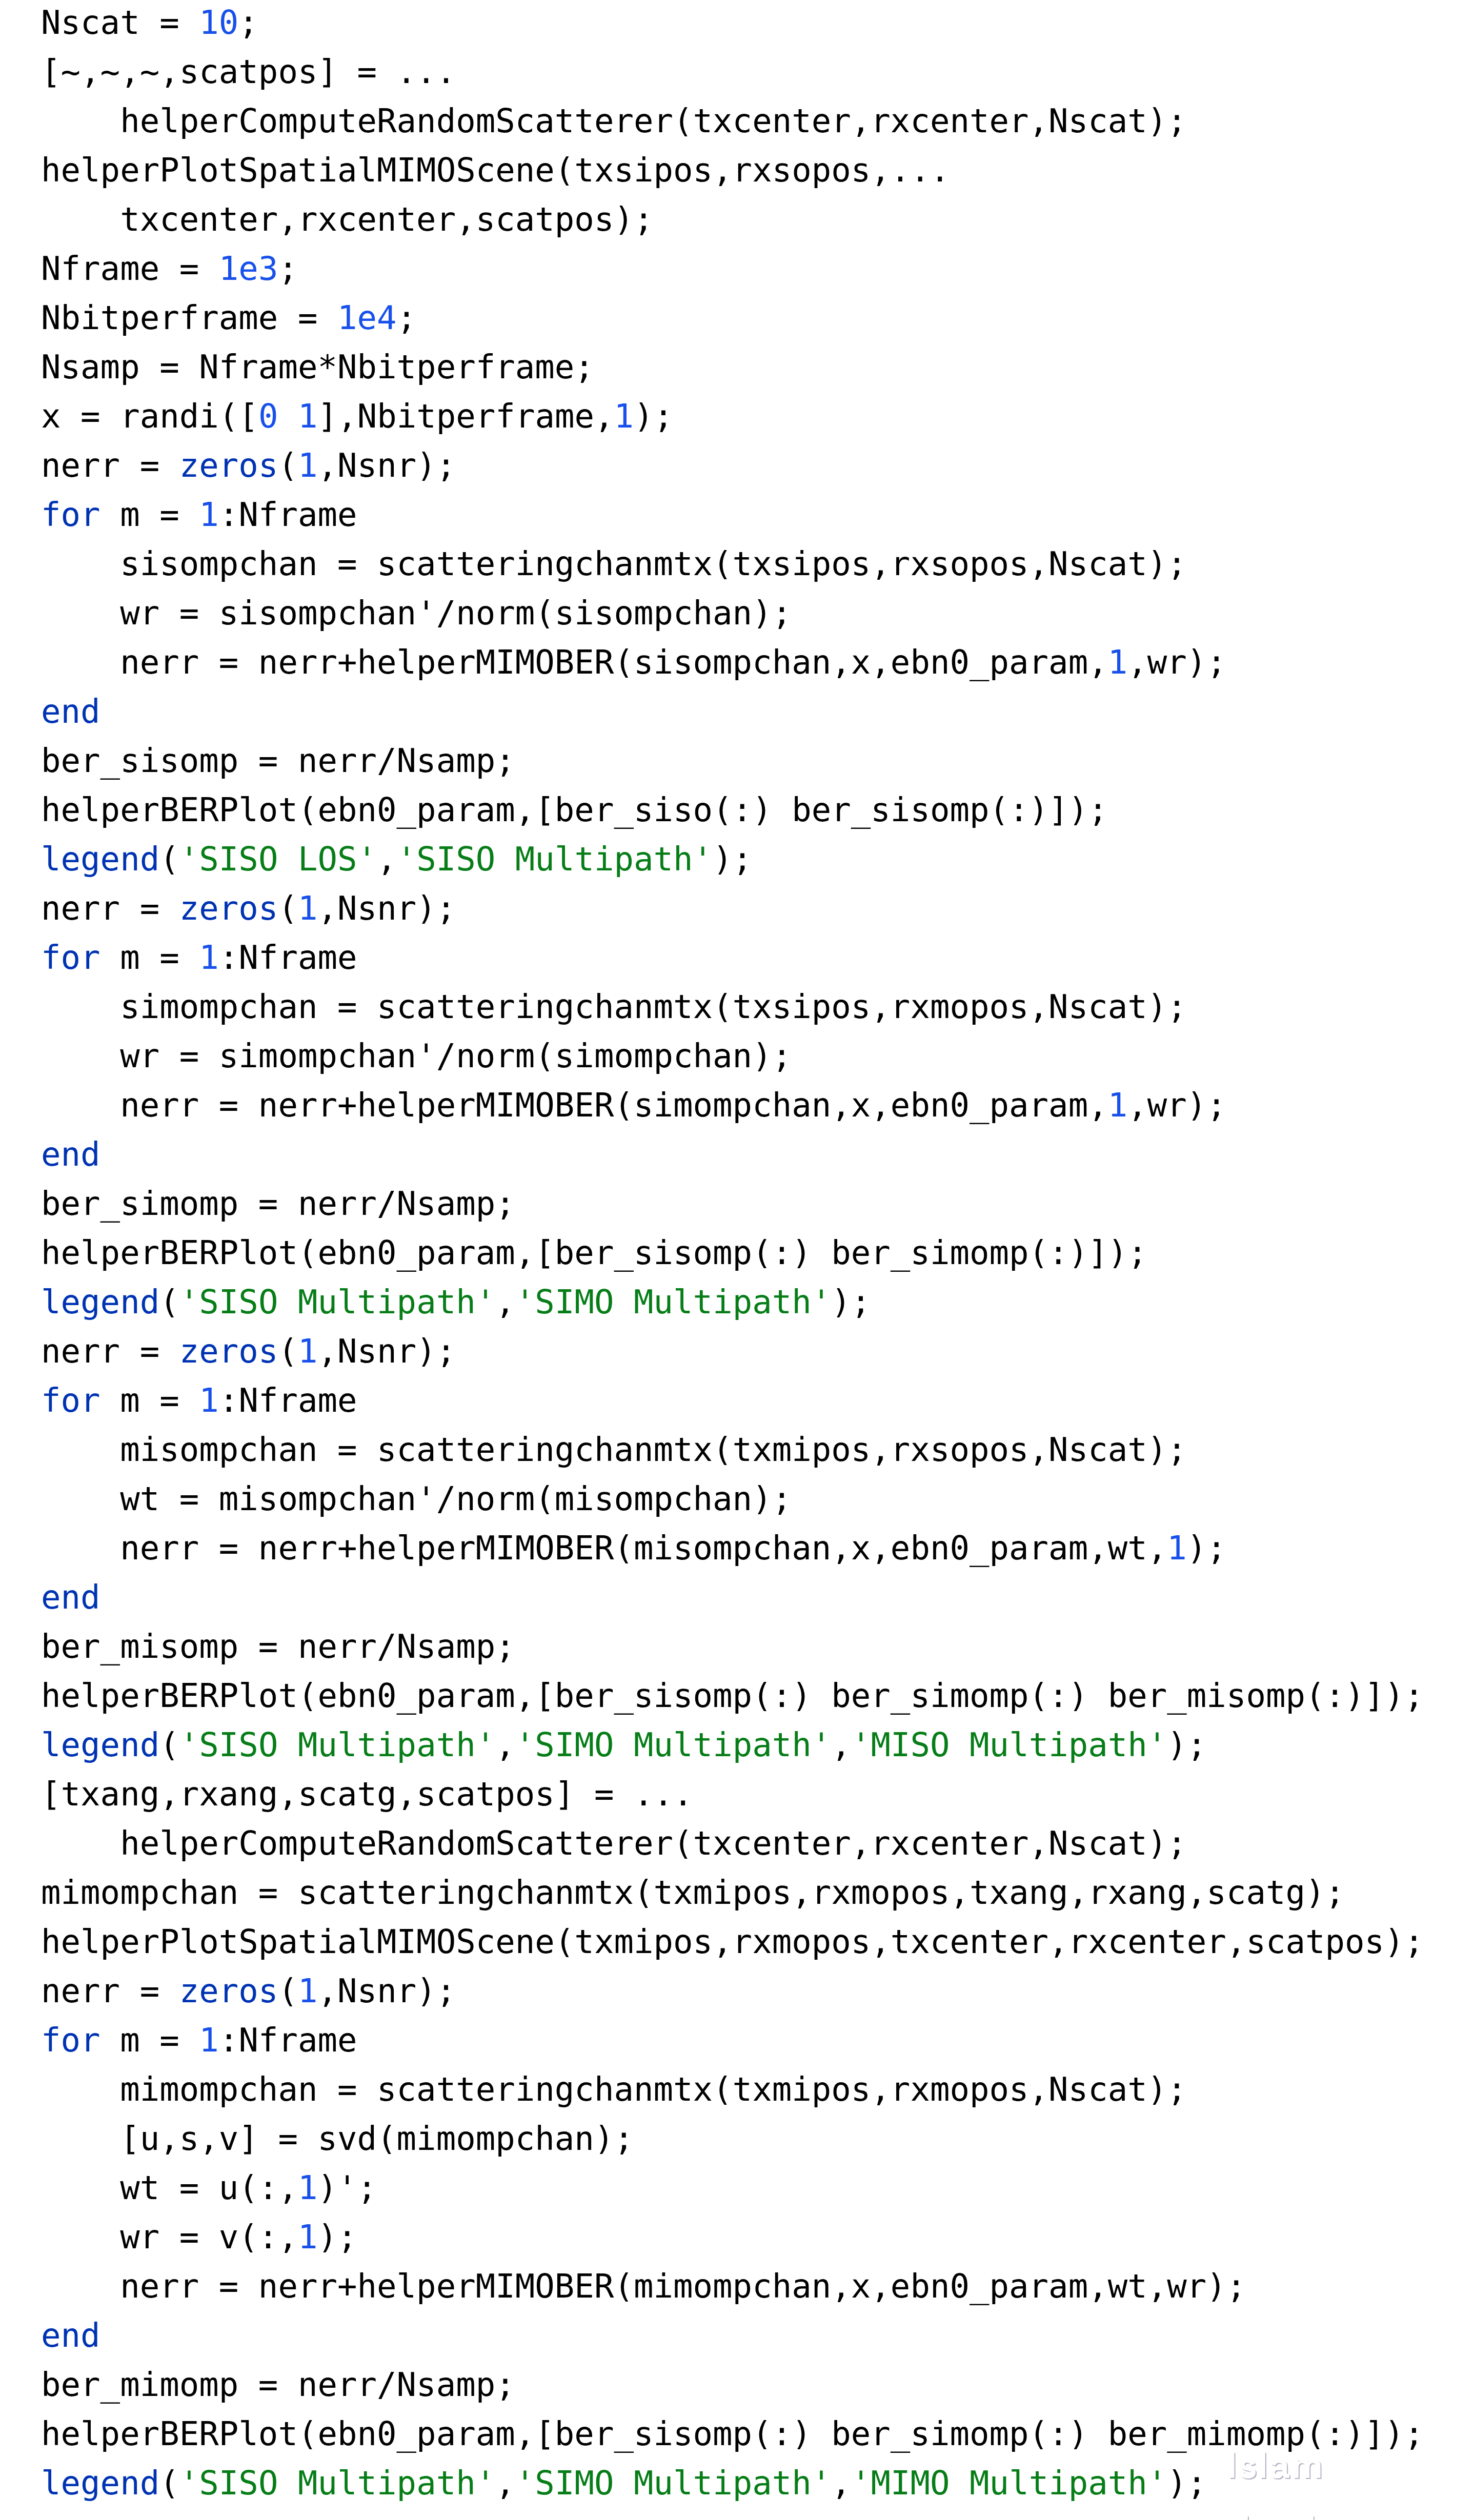
\includegraphics[width=0.8\linewidth]{figures/fullcode3}
\end{figure}
\restoregeometry
%\input{appendix/appendix-b}
%\input{appendix/appendix-c} % Create file to add

\end{document}
